


\section{Clustering of the typical point in $\Ginf$\label{sec:Ginf}\label{sec:asymptotics_average_clustering_ast_P}}


Similar to the proof for the degrees we plan to make use of the Campbell-Mecke formula for comparing the clustering coefficient and function of $\GPo$ with certain quantities associated with $\Ginf$. Recall that a \emph{typical point} is a point $p_0 = (0,y)$, where in some computations the height $y$ will be fixed, but eventually we shall take it exponentially distributed with parameter $\alpha$, and independent of $\Pcal$.

Since $c(G)$ is defined as an average over all vertices of the graph, it is not immediately obvious how to meaningfully define a corresponding notion for infinite graphs, and similarly for the clustering function, the degree sequence, etc.
We can however without any issues speak of the (expected) clustering coefficient of the typical point or the expected clustering coefficient given that it has degree $k$. (All considered in the graph obtained from $\Ginf$ by adding the typical point to its vertex set.)

If $p = (x,y) \in \eR\times[0,\infty)$ is a point, not necessarily part of the Poisson process, then we write
\[ 
	\mu(y) = \mu(p) := \mu(\BallPo{p}).
\]
Recall that $\mu(y) = \frac{2\alpha \nu e^{y/2}}{\pi(\alpha-\frac12)} = \xi e^{y/2}$. When $p = (0,y)$ we also write $\BallPo{y} = \BallPo{p}$.


\subsection{The expected clustering coefficient and function of the typical point}


Let the random variable $C$ denote the clustering coefficient of the typical point $(0,y)$, in the graph obtained from $\Ginf$ by adding $(0,y)$. We now {\em define}
\[
	\gamma := \Exp{C}, \quad \gamma(k) := \CExp{C}{D = k}.
\]
(Where we take the expectation over both the Poisson point process $\Pcal$ and $y \isd \text{exp}(\alpha)$, independently of the Poisson process $\Pcal$.) We shall show shortly that these take on the values stated in Theorem~\ref{thm:maincc} and~\ref{thm:mainkfixed}.


For any fixed value $y_0>0$, the set of points inside $\BallPo{y_0}$ is a Poisson process with intensity $f \cdot 1_{\BallPo{y_0}}$. As $\mu(\BallPo{y_0}) = \mu(y_0) = \xi e^{y_0/2} < \infty$, this can be described alternatively by first picking $N \isd \Po( \mu(y_0) )$ and then taking $N$ i.i.d.~points in $\BallPo{y_0}$ according to the probability density $f \cdot 1_{\BallPo{y_0}} / \mu(y_0)$. (That is, the intensity function of the Poisson point process, but set to zero outside of $\BallPo{y_0}$ and re-normalized in such a way that it integrates to one.) Hence, if we condition on the event that $y$ takes on some fixed value $y_0$ and that there are exactly $k$ points of $\Pcal$ inside $\BallPo{y_0}$, then those $k$ points behave like $k$ i.i.d.~points in $\BallPo{y_0}$ chosen according to the mentioned re-normalized probability density function. This shows that, for every $k\geq 2$:
\[
	\CExp{C}{D=k, y=y_0} 
	= \frac{1}{{k\choose 2}} \Ee\left( \sum_{1\leq i < j \leq k} \1_{\{u_i\in \BallPo{u_j}\}} \right)
	= \Exp{\1_{\{u_1\in\BallPo{u_2}\}}},
\]
where $u_1,\dots, u_n$ are i.i.d.~points in $\BallPo{y_0}$ with the above mentioned density.
Note that this does not depend on the value of $k$. For notational convenience, we will write 
\[ 
	P(y_0) := \Exp{\1_{\{u_1\in\BallPo{u_2}\}}},
\]
with $u_1, u_2$ as above.

We now observe that 
\[
	\gamma(k) = \CExp{C}{D=k} = \int_0^\infty \CExp{C}{D=k, y=y_0} g_k(y_0) \, d y_0,
\]
where $g_k$ denotes the density of $y$ {\em conditional on} $D=k$. That is,
\[
	g_k(y_0)  = \frac{\rho(y_0, k) \alpha e^{-\alpha y_0} }{\int_0^\infty \rho(t, k) \alpha e^{-\alpha t} \, d t}
	= \frac{1}{p_k} \cdot \rho(y_0, k) \alpha e^{-\alpha y_0},
\]
where we recall that $\rho(y,k) = \Prob{\Po(\mu(y)) = k}$ denotes the probability that a Poisson random variable with mean $\mu(y)$ is $k$. Hence, 
\begin{equation}\label{eq:gammakint}
\gamma(k) 
= \frac{1}{p_k} \cdot \int_0^\infty P(y_0) \rho(y_0,k) \alpha e^{-\alpha y_0} \, d y_0. 
\end{equation}
This also gives
\begin{equation}\label{eq:gammaint}
\begin{array}{rcl} 
\gamma 
& = & \displaystyle \Exp{C} = \sum_{k\geq 2} \CExp{ C }{ D=k }\Prob{ D=k } \\
& = & \displaystyle \int_0^\infty P(y_0) \left( \sum_{k=2}^\infty \rho(y_0,k) \right) \alpha e^{-\alpha y_0} \, d y_0 \\
& = & \displaystyle \int_0^\infty P(y_0) \left(1 - \rho(y_0,0)-\rho(y_0,1)\right) \alpha e^{-\alpha y_0} \, d y_0.
\end{array}
\end{equation}


A key step is to derive the following explicit expression for $P(y)$.

\begin{lemma}\label{lem:Paneq1}
%\begin{enumerate}
%	\item 
	If $\alpha \not = 1$, then
	\begin{align*}
	 P(y) &=-\frac{1}{8 (\alpha - 1) \alpha} + \frac{(\alpha - 1/2) e^{-\frac{1}{2}y}}{\alpha - 1} - \frac{(\alpha - 1/2)^2 e^{-y}}{
		4 (\alpha - 1)^2} \\
	&+ 
	(e^{-\frac{1}{2}y})^{4\alpha -2} \left(\frac{2^{-4 \alpha-1} (3 \alpha - 1)}{\alpha (\alpha - 1)^2} 
		+ \frac{(\alpha - 1/2 ) B^-(1/2; 1 + 2 \alpha, -2 + 2 \alpha)}{2(\alpha - 1) \alpha} \right) \\
	&+ \frac{(1 - 
		e^{-\frac{1}{2}y})^{2 \alpha}}{8 (\alpha - 1) \alpha} - \frac{  
		(e^{-\frac{1}{2}y})^{4 \alpha - 2} B^-(1 - e^{-\frac{1}{2}y}; 2 \alpha, 3 - 4 \alpha)}{4 (\alpha - 1)}
	\end{align*}
% 	\item If $\alpha = 1$, then
% 	\begin{align*}
% 	&P(y) =\frac{9}{4} e^{-\frac{1}{2}y} + \frac{1 - 4 e^{-\frac{1}{2}y} + 3 e^{-y}}{4}\ln(1 - e^{-\frac{1}{2}y}) - \frac{7+\pi^2}{8}
% e^{-y}  + 
% \frac{1}{2}e^{-y}\Li_2(e^{-y})
% 	\end{align*}
% 	where $\Li_2(z)=\int_0^z \frac{\ln(1-t)}{t}dt$ is the dipolylogarithm function.
%\end{enumerate}
\end{lemma}


We will prove this lemma in a sequence of steps.

Recall that $P(y_0)$ is the probability that $u_1 = (x_1,y_1), u_2 = (x_2,y_2)$ are neighbours in $\Ginf$, where
$u_1, u_2$ are i.i.d.~with probability density $f \cdot \1_{\BallPo{y_0}} / \mu(y_0)$.
In particular
\begin{align*}
	\Prob{y_i > t} &= \frac{\nu\alpha}{\pi \mu(y_0)} \int_t^\infty \int_{-e^{(y+y_0)/2}}^{e^{(y+y_0)/2}} e^{-\alpha y}
		\dd x \dd y
		= \frac{\nu\alpha}{\pi \mu(y_0)} \int_t^\infty 2 e^{(y+y_0)/2} \cdot e^{-\alpha y} \dd y \\
	&= \frac{2 \nu\alpha e^{y_0/2} }{\pi \xi e^{y_0/2} (\alpha-\frac{1}{2}) }  \cdot e^{(\frac{1}{2}-\alpha)t}
		= e^{(\frac{1}{2}-\alpha)t},
\end{align*}
using that $\mu(y_0) = \xi e^{y_0/2} = \left(\frac{2\alpha\nu}{\pi(\alpha-\frac12)}\right) e^{y_0/2}$.
Thus, $y_1, y_2$ are exponentially distributed with parameter $\alpha-\frac12$.
Now note that, for each $t>0$, the probability density $f \cdot 1_{\BallPo{y_0}} / \mu(y_0)$
is constant on $[-e^{(t+y_0)/2}, e^{(t+y_0)/2}] \times \{t\}$ and it is 
vanishes on $(-\infty, -e^{(t+y_0)/2}) \times \{t\} \cup (e^{(t+y_0)/2},\infty)\times\{t\}$.

Hence, given the height $y_i$ of $u_i$, the $x$-coordinate of $u_i$ is uniform in $[-e^{\frac{1}{2}(y+y_i)},e^{\frac{1}{2}(y+y_i)}]$. 
With this in mind we define $P(y_0,y_1,y_2)$ to be the probability that $y_0, (x_1,y_1), (x_2,y_2)$ 
satisfy \\ $|x_1-x_2| \leq e^{(y_1+y_2)/2}$, where $x_1$ and $x_2$ are independent uniform random variables in the intervals
$[-e^{\frac{1}{2}(y_0+y_1)},e^{\frac{1}{2}(y_0+y_1)}]$ and  $[-e^{\frac{1}{2}(y_0+y_2)},e^{\frac{1}{2}(y_0+y_2)}]$, respectively. We then have that
\begin{equation}\label{eq:delta_P}
 P(y_0) = (\alpha-1/2)^2 \int_0^\infty \int_0^\infty P(y_0, y_1, y_2) e^{-(\alpha-1/2)(y_1+y_2)} 
 \dd y_2 \dd y_1.
\end{equation}

\subsubsection{Determining $P(y_0,y_1,y_2)$}


To compute the integral~\eqref{eq:delta_P} it will be convenient to use the 
change of variable $z_i = e^{-y_i/2}$, for $i= 0, 1, 2$. 
We will write $y_i(z_i)$ to stress the dependence between $y_i$ and $z_i$. 
The following result completely characterizes $P(y_0,y_1,y_2)$.

\begin{lemma}\label{lem:triangle_prob_y_coordinates}
\begin{align*}
P(y_0(z_0),y_1(z_1),y_2(z_2)) = \begin{cases}
	1, &\text{ if } z_0 \geq z_1+z_2, z_0 > z_1 > z_2, \\
	1-G(z_0,z_1,z_2), &\text{ if } z_0 < z_1+z_2, z_0 > z_1 > z_2, \\
	\frac{z_0}{z_1}, &\text{ if } z_1 \geq z_0+z_2, z_1 > \max(z_0,z_2), \\
	\frac{z_0}{z_1}\left(1-G(z_1,z_0,z_2)\right), &\text{ if } z_1 < z_0+z_2, z_1 > \max(z_0,z_2),
\end{cases}
\end{align*}
where 
\begin{align*}
G(a,b,c) = \frac{1}{4}
\left( b^{-1}c + bc^{-1} + a^2b^{-1}c^{-1} + 2 - 2ab^{-1}-2ac^{-1}\right).
\end{align*}
\end{lemma}


%\begin{align*}
%G'(z_0,z_1,z_2) = \frac14 ( z_1^{-1} z_2 +z_0^2 z_1^{-1} z_2^{-1} + z_1 z_2^{-1} + 2z_0z_1^{-1} - 2 - 2z_0z_2^{-1} )
%\end{align*}

We split the proof of this lemma into a couple of smaller pieces. We begin with the following lemma.

\begin{lemma}\label{lem:ordered}
Let $z_i = e^{-y_i/2}$, $i=0,1,2$. If $y_0<y_1<y_2$ (or equivalently $z_0 > z_1 > z_2$), then
\begin{align*}
P(y_0(z_0),y_1(z_1),y_2(z_2)) = \begin{cases}
1, &\text{ if } z_0 \geq z_1+z_2,  \\
1-G(z_0,z_1,z_2), &\text{ if } z_0 < z_1+z_2
\end{cases}
\end{align*}
\end{lemma}

\begin{figure}[!t]
\centering
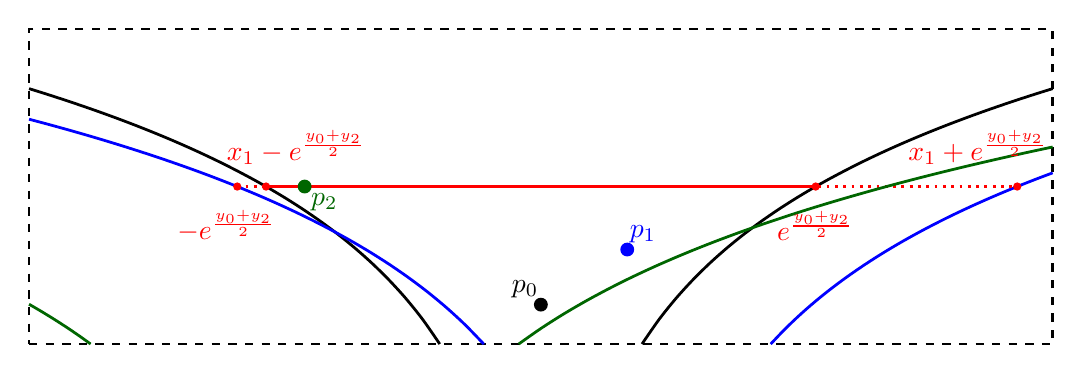
\begin{tikzpicture}
	%Define the coordinates 
	%p = (\u,\v) and p^\prime = (\uu, \vv)
	%Box \Rcal_n has width 2\r and height \t
	\pgfmathsetmacro{\u}{0} %0
	\pgfmathsetmacro{\v}{0.5} %1
	\pgfmathsetmacro{\vv}{1.2} %0.8
	\pgfmathsetmacro{\vvv}{2} %0.8
	\pgfmathsetmacro{\uuu}{-3} %1.4	
	\pgfmathsetmacro{\r}{6.5}
	\pgfmathsetmacro{\t}{4}
	
	\pgfmathsetmacro{\ubound}{exp((\vv+\vvv)/2)-exp((\v+\vvv)/2)}
	
	\pgfmathsetmacro{\uu}{3*\ubound/4}
	
	\pgfmathsetmacro{\leftintvandvvv}{-exp((\v + \vvv)/2)}
	\pgfmathsetmacro{\rightintvandvvv}{exp((\v + \vvv)/2)}
	\pgfmathsetmacro{\leftintvvandvvv}{\uu-exp((\vv + \vvv)/2)}
	\pgfmathsetmacro{\rightintvvandvvv}{\uu+exp((\vv + \vvv)/2)}
		
	%The box \Rcal_n
	\draw[line width=1pt,dashed] (-\r,0) -- (\r,0) -- (\r,\t) -- (-\r,\t) -- (-\r,0);

	%Dram all three nodes
    \draw node[fill, circle, inner sep=0pt, minimum size=5pt] (p1) at (\u,\v) {};
    \path (p1)+(-0.2,0.2) node {$p_0$};
    \draw node[fill,blue, circle, inner sep=0pt, minimum size=5pt] (p2) at (\uu,\vv) {};
    \path (p2)+(0.2,0.2) node {\color{blue}$p_1$};	
	
	%Boundaries p_0 = (\u,\v)
	
	%Right boundary
	\pgfmathsetmacro{\rightbounduv}{\u+exp((\v)/2)}
	\draw[domain=\rightbounduv:\r,smooth,variable=\x,black,line width=1pt] plot (\x, {2*ln(\x)-\v});
    %Left boundary
    \pgfmathsetmacro{\leftbounduv}{\u-exp((\v)/2)}
    \draw[domain=\leftbounduv:-\r,smooth,variable=\x,black,line width=1pt] plot (\x, {2*ln(-\x)-\v});
    
    %Boundaries p_1 = (\uu,\vv)
    
    %Right boundary
    \pgfmathsetmacro{\rightbounduuvv}{\uu+exp((\vv)/2)}
    \draw[domain=\rightbounduuvv:\r,smooth,variable=\x,blue,line width=1pt] plot (\x, {2*ln(\x-\uu)-\vv});
%    %Shifted right boundary
%    \pgfmathsetmacro{\shiftrightbounduuvv}{\uu+exp((\vv + \t)/2)-2*\r}
%    \draw[domain=\shiftrightbounduuvv:-\r,smooth,variable=\x,blue,line width=1pt] plot (\x, {2*ln(\x+(2*\r-\uu))-\vv});
    %Left boundary 
    \pgfmathsetmacro{\leftbounduuvv}{\uu-exp((\vv)/2)}
    \draw[domain=\leftbounduuvv:-\r,smooth,variable=\x,blue,line width=1pt] plot (\x, {2*ln(\uu-\x)-\vv});
%    %Shifted left boundary
%    \pgfmathsetmacro{\shiftleftbounduuvv}{\uu-exp((\vv + \t)/2)+2*\r}
%    \draw[domain=\shiftleftbounduuvv:\r,smooth,variable=\x,blue,line width=1pt] plot (\x, {2*ln(2*\r + \uu-\x)-\vv});
   


	\draw [red,dotted,line width=1pt] (\leftintvandvvv,\vvv) -- (\rightintvandvvv,\vvv);
	
	\draw [red,dotted,line width=1pt] (\leftintvvandvvv,\vvv) -- (\rightintvvandvvv,\vvv);

	\draw [red,line width=1pt] (\leftintvandvvv,\vvv) -- (\rightintvandvvv,\vvv);

    \draw node[fill,black!60!green, circle, inner sep=0pt, minimum size=5pt] (p2) at (\uuu,\vvv) {};
    \path (p2)+(0.25,-0.2) node {\color{black!60!green}$p_2$};
    
	%Boundaries p_2 = (\uuu,\vvv)
	
	%Right boundary
	\pgfmathsetmacro{\rightbounduuuvvv}{\uuu+exp((\vvv)/2)}
	\draw[domain=\rightbounduuuvvv:\r,smooth,variable=\x,black!60!green,line width=1pt] plot (\x, {2*ln(\x-\uuu)-\vvv});
    %Left boundary
    \pgfmathsetmacro{\leftbounduuuvvv}{\uuu-exp((\vvv)/2)}
    \draw[domain=\leftbounduuuvvv:-\r,smooth,variable=\x,black!60!green,line width=1pt] plot (\x, {2*ln(\uuu-\x)-\vvv});

	\draw node[fill,red, circle, inner sep=0pt, minimum size=3pt] at (\leftintvandvvv,\vvv) {};
	\path (\leftintvandvvv,\vvv)+(-0.5,-0.5) node[red] {$-e^{\frac{y_0 + y_2}{2}}$};
	\draw node[fill,red, circle, inner sep=0pt, minimum size=3pt] at (\rightintvandvvv,\vvv) {};
	\path (\rightintvandvvv,\vvv)+(0,-0.5) node[red] {$e^{\frac{y_0 + y_2}{2}}$};
	
	\draw node[fill,red, circle, inner sep=0pt, minimum size=3pt] at (\leftintvvandvvv,\vvv) {};
	\path (\leftintvvandvvv,\vvv)+(0.75,0.5) node[red] {$x_1 - e^{\frac{y_0 + y_2}{2}}$};
	\draw node[fill,red, circle, inner sep=0pt, minimum size=3pt] at (\rightintvvandvvv,\vvv) {};
	\path (\rightintvvandvvv,\vvv)+(-0.5,0.5) node[red] {$x_1 + e^{\frac{y_0 + y_2}{2}}$};

\end{tikzpicture}\\
\vspace{0.5cm}
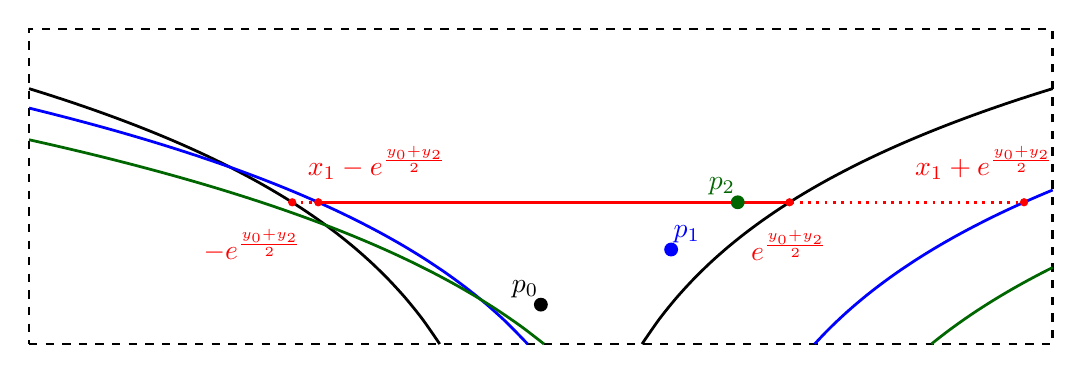
\begin{tikzpicture}
	%Define the coordinates 
	%p = (\u,\v) and p^\prime = (\uu, \vv)
	%Box \Rcal_n has width 2\r and height \t
	\pgfmathsetmacro{\u}{0} %0
	\pgfmathsetmacro{\v}{0.5} %1
	\pgfmathsetmacro{\vv}{1.2} %0.8
	\pgfmathsetmacro{\vvv}{1.8} %0.8
	\pgfmathsetmacro{\uuu}{2.5} %1.4	
	\pgfmathsetmacro{\r}{6.5}
	\pgfmathsetmacro{\t}{4}
	
	\pgfmathsetmacro{\ubound}{exp((\vv+\vvv)/2)-exp((\v+\vvv)/2)}
	
	\pgfmathsetmacro{\uu}{5*\ubound/4}
	
	\pgfmathsetmacro{\leftintvandvvv}{-exp((\v + \vvv)/2)}
	\pgfmathsetmacro{\rightintvandvvv}{exp((\v + \vvv)/2)}
	\pgfmathsetmacro{\leftintvvandvvv}{\uu-exp((\vv + \vvv)/2)}
	\pgfmathsetmacro{\rightintvvandvvv}{\uu+exp((\vv + \vvv)/2)}
		
	%The box \Rcal_n
	\draw[line width=1pt,dashed] (-\r,0) -- (\r,0) -- (\r,\t) -- (-\r,\t) -- (-\r,0);

	%Dram all three nodes
    \draw node[fill, circle, inner sep=0pt, minimum size=5pt] (p1) at (\u,\v) {};
    \path (p1)+(-0.2,0.2) node {$p_0$};
    \draw node[fill,blue, circle, inner sep=0pt, minimum size=5pt] (p2) at (\uu,\vv) {};
    \path (p2)+(0.2,0.2) node {\color{blue}$p_1$};	
	
	%Boundaries p_0 = (\u,\v)
	
	%Right boundary
	\pgfmathsetmacro{\rightbounduv}{\u+exp((\v)/2)}
	\draw[domain=\rightbounduv:\r,smooth,variable=\x,black,line width=1pt] plot (\x, {2*ln(\x)-\v});
    %Left boundary
    \pgfmathsetmacro{\leftbounduv}{\u-exp((\v)/2)}
    \draw[domain=\leftbounduv:-\r,smooth,variable=\x,black,line width=1pt] plot (\x, {2*ln(-\x)-\v});
    
    %Boundaries p_1 = (\uu,\vv)
    
    %Right boundary
    \pgfmathsetmacro{\rightbounduuvv}{\uu+exp((\vv)/2)}
    \draw[domain=\rightbounduuvv:\r,smooth,variable=\x,blue,line width=1pt] plot (\x, {2*ln(\x-\uu)-\vv});
    %Left boundary 
    \pgfmathsetmacro{\leftbounduuvv}{\uu-exp((\vv)/2)}
    \draw[domain=\leftbounduuvv:-\r,smooth,variable=\x,blue,line width=1pt] plot (\x, {2*ln(\uu-\x)-\vv});


	\draw [red,dotted,line width=1pt] (\leftintvandvvv,\vvv) -- (\rightintvandvvv,\vvv);
	
	\draw [red,dotted,line width=1pt] (\leftintvvandvvv,\vvv) -- (\rightintvvandvvv,\vvv);

	\draw [red,line width=1pt] (\leftintvvandvvv,\vvv) -- (\rightintvandvvv,\vvv);
	


    \draw node[fill,black!60!green, circle, inner sep=0pt, minimum size=5pt] (p2) at (\uuu,\vvv) {};
    \path (p2)+(-0.2,0.2) node {\color{black!60!green}$p_2$};
    
	%Boundaries p_2 = (\uuu,\vvv)
	
	%Right boundary
	\pgfmathsetmacro{\rightbounduuuvvv}{\uuu+exp((\vvv)/2)}
	\draw[domain=\rightbounduuuvvv:\r,smooth,variable=\x,black!60!green,line width=1pt] plot (\x, {2*ln(\x-\uuu)-\vvv});
    %Left boundary
    \pgfmathsetmacro{\leftbounduuuvvv}{\uuu-exp((\vvv)/2)}
    \draw[domain=\leftbounduuuvvv:-\r,smooth,variable=\x,black!60!green,line width=1pt] plot (\x, {2*ln(\uuu-\x)-\vvv});

	\draw node[fill,red, circle, inner sep=0pt, minimum size=3pt] at (\leftintvandvvv,\vvv) {};
	\path (\leftintvandvvv,\vvv)+(-0.5,-0.55) node[red] {$-e^{\frac{y_0 + y_2}{2}}$};
	\draw node[fill,red, circle, inner sep=0pt, minimum size=3pt] at (\rightintvandvvv,\vvv) {};
	\path (\rightintvandvvv,\vvv)+(0,-0.55) node[red] {$e^{\frac{y_0 + y_2}{2}}$};
	
	\draw node[fill,red, circle, inner sep=0pt, minimum size=3pt] at (\leftintvvandvvv,\vvv) {};
	\path (\leftintvvandvvv,\vvv)+(0.75,0.5) node[red] {$x_1 - e^{\frac{y_0 + y_2}{2}}$};
	\draw node[fill,red, circle, inner sep=0pt, minimum size=3pt] at (\rightintvvandvvv,\vvv) {};
	\path (\rightintvvandvvv,\vvv)+(-0.5,0.5) node[red] {$x_1 + e^{\frac{y_0 + y_2}{2}}$};

\end{tikzpicture}
\caption{Situation for the intersections of the connection intervals considered in Lemma~\ref{lem:ordered}, with $y_0 < y_1 <y_2$ fixed and for different cases of $0 \le x_1 \le e^{(y_0 + y_1)/2}$. The top figure shows the case where $0 \le x_1 \le e^{(y_1 + y_2)/2} - e^{(y_0 + y_2)/2}$, while the bottom one shows the case $x_1 > e^{(y_1 + y_2)/2} - e^{(y_0 + y_2)/2}$. The solid red line indicates the range for $x_2$ such that the points $p_0$, $p_1$ and $p_2$ form a triangle. The boundaries of their neighbourhoods are shown in, respectively, black, blue and green.}
\label{fig:triangle_prob_lemma}
\end{figure}

\begin{proof}
Note that $P(y_0,y_1,y_2)$ is the probability that $x_2$ falls into the interval $[x_1-e^{(y_1+y_2)/2},x_1+e^{(y_1+y_2)/2}]$, as well as into the interval $[-e^{(y_0+y_2)/2},e^{(y_0+y_2)/2}]$. By symmetry considerations, we can take $x_1$ uniformly at random from $[0,e^{y_0/2+y_1/2}]$ as opposed to $[-e^{y_0/2+y_1/2}, e^{y_0/2+y_1/2}]$. Figure~\ref{fig:triangle_prob_lemma} shows the intersection of the intervals (red line) for two different cases for $x_1 \le e^{(y_0 + y_1)/2}$. 

Since $y_0 < y_1 < y_2$ we have that $e^{(y_1+y_2)/2} > e^{(y_0+y_2)/2}$ and so, when $x_1 \geq 0$, the ``right half'' of the 
interval $[-e^{(y_0+y_2)/2}, e^{(y_0+y_2)/2}]$ is always covered by the interval $[x_1-e^{(y_1+y_2)/2}, x_1+e^{(y_1+y_2)/2}]$.
If $e^{(y_1+y_2)/2} - e^{(y_0+y_1)/2} \geq e^{(y_0+y_2)/2}$ then the ``left half'' is always covered as well.
In other words:
\[
	e^{(y_1+y_2)/2} - e^{(y_0+y_1)/2} \geq e^{(y_0+y_2)/2} \Rightarrow P(y_0,y_1,y_2) = 1.
\]

Now consider the case where $e^{(y_1+y_2)/2} - e^{(y_0+y_1)/2} < e^{(y_0+y_2)/2}$. 
Then, if $x_1 \in [0, e^{(y_1+y_2)/2} - e^{(y_0+y_2)/2}]$ the whole interval $[-e^{(y_0+y_2)/2}, e^{(y_0+y_2)/2}]$ is still covered 
so that $p_0, p_1$ and $p_2$ form a triangle. If, on the other hand $e^{(y_1+y_2)/2} - e^{(y_0+y_2)/2} < x_1 \leq e^{(y_0+y_1)/2}$ then
the probability that $|x_2-x_1| \leq e^{(y_1+y_2)/2}$ equals
\[ 
	1 - \frac{x_1 - (e^{(y_1+y_2)/2} - e^{(y_0+y_2)/2)}) }{ 2e^{(y_0+y_2)/2} }. 
\]

Hence, when $e^{(y_1+y_2)/2} - e^{(y_0+y_1)/2} < e^{(y_0+y_2)/2}$ we have
\begin{align*}
	P(y_0,y_1,y_2) &= \frac{e^{(y_1+y_2)/2} - e^{(y_0+y_2)/2} }{ e^{(y_0+y_1)/2} }  \\
	&\hspace{10pt}+ \int_{ e^{(y_1+y_2)/2} - e^{(y_0+y_2)/2} }^{ e^{(y_0+y_1)/2} } 
	    \left(1 - \frac{x_1 - (e^{(y_1+y_2)/2} - e^{(y_0+y_2)/2)}) }{ 2e^{(y_0+y_2)/2} }\right)
	    \cdot \frac{1}{e^{(y_0+y_1)/2}} \dd x_1 \\
	&= 1 - \frac{1}{2e^{y_0+y_1/2+y_2/2} } \int_0^{ e^{(y_0+y_1)/2}+e^{(y_0+y_2)/2}-e^{(y_1+y_2)/2} } x_1 \dd x_1 \\
	&= 1 - \frac{ \left( e^{(y_0+y_1)/2}+e^{(y_0+y_2)/2}-e^{(y_1+y_2)/2} \right)^2 }{ 4 e^{y_0+y_1/2+y_2/2} }.
\end{align*}

At this point it is convenient to rewrite everything in terms of $z_i := e^{-y_i/2}$.
Note that $y_0 < y_1 < y_2$ if and only if $z_0 > z_1 > z_2$ while the condition $e^{(y_1+y_2)/2} - e^{(y_0+y_1)/2} < e^{(y_0+y_2)/2}$ becomes
\[ e^{(y_1+y_2)/2} - e^{(y_0+y_1)/2} < e^{(y_0+y_2)/2} \Leftrightarrow 
z_1^{-1} z_2^{-1} < z_0^{-1} z_1^{-1} + z_0^{-1}z_2^{-1} 
\Leftrightarrow
z_0 < z_1+z_2. 
\]

We now conclude that
\[
	P(y_0(z_0), y_1(z_1), y_2(z_2)) = 1 \quad \text{if} \quad z_0 > z_1 > z_2 \text{ and } z_0 \geq z_1 + z_2
\]
while for $z_0 > z_1 > z_2$ and $z_0 < z_1 + z_2$
\begin{align*}
	P(y_0(z_0), y_1(z_1), y_2(z_2)) 
	&= 1 - \frac{z_0^2z_1z_2}{4} \cdot \left( z_0^{-1}z_1^{-1}+z_0^{-1}z_2^{-1}-z_1^{-1}z_2^{-1} \right)^2 \\
%	&= 1 - \frac{z_0^2z_1z_2}{4} \cdot \left( z_0^{-2}z_1^{-2} + z_0^{-2}z_2^{-2} + z_1^{-2}z_2^{-2}
%		+ 2z_0^{-2}z_1^{-1}z_2^{-1} - 2 z_0^{-1}z_1^{-2}z_2^{-1} - 2z_0^{-1}z_1^{-1}z_2^{-2} \right) \\
	&= 1 - \frac{1}{4} \left( z_1^{-1}z_2 + z_1z_2^{-1} + z_0^2z_1^{-1}z_2^{-1} + 2 - 2z_0z_1^{-1}-2z_0z_2^{-1}\right),
\end{align*}
which finishes the proof.
\end{proof}

The previous lemma covers the case when $y_0<y_1<y_2$. We now leverage it to take care of the other cases as well. 

\begin{proof}[Proof of Lemma~\ref{lem:triangle_prob_y_coordinates}]
Let $y_i >0$ and $z_i = e^{-y_i/2}$, $i=0,1,2$. Lemma~\ref{lem:ordered} gives the expression for $P(y_0(z_0),y_1(z_1),y_2(z_2))$ in the case $y_0<y_1<y_2$, or equivalently $z_0>z_1>z_2$, i.e. the first two lines in the claim of Lemma~\ref{lem:triangle_prob_y_coordinates}. To analyze the other cases we shall express $P(y_1,y_0,y_2)$ and $P(y_1,y_2,y_0)$ in terms of $P(y_0,y_1,y_2)$ and $z_i$. For this we note that we can view $P(y_0,y_1,y_2)$ as a 2-fold integral of the indicator function
\[ 
	h(x_0, x_1, x_2) := \ind{ |x_0 - x_1| < e^{(y_0+y_1)/2}, |x_0 - x_2| < e^{(y_0+y_2)/2}, |x_1-x_2| < e^{(y_1+y_2)/2}}, 
\]
where $x_0$ was set to zero, without loss of generality, and the other two $x_i$ are uniform random variables on $[-e^{(y_0+y_i)/2}, e^{(y_0+y_i)/2}]$. When we consider the probability $P(y_1,y_0,y_2)$, this is the 2-fold integral of $h(x_0,0,x_2)$ so that
\begin{align*}
	P(y_1,y_0,y_2) &= \frac{1}{2e^{(y_1+y_0)/2}} \cdot \frac{1}{2e^{(y_1+y_2)/2}} 
		\iint_{\R} h(x_0,0,x_2) \dd x_0 \dd x_2\\
	&= \frac{e^{y_0/2}}{e^{y_1/2}} \frac{1}{2e^{(y_0+y_1)/2}} \frac{1}{2e^{(y_0+y_2)/2}} 
		\iint_{\R} h(0,x_1,x_2) \dd x_1 \dd x_2\\
	&= \frac{e^{y_0/2}}{e^{y_1/2}} P(y_0,y_1,y_2) = \frac{z_1}{z_0}  P(y_0,y_1,y_2).
\end{align*}
Finally we note that $h(x_0,0,x_2) = h(x_2,0,x_0)$ from which we conclude that
\begin{equation}\label{eq:symmetry_relation_triangle_prob}
	P(y_0, y_1, y_2) = \left(z_0/z_1\right) P(y_1,y_0,y_2) = \left(z_0/z_1\right) P(y_1,y_2,y_0).
\end{equation}

To complete the proof for the other cases we note that since $P(y_0,y_1,y_2)$ is symmetric in $y_1$ and $y_2$, we can assume, without loss of generality, that $y_1 < y_2$. Then, there are two more orderings of $y_0, y_1, y_2$, namely $y_1< y_0< y_2$ and $y_1<y_2<y_0$, which can be summarized as $y_1 < \min (y_0,y_2)$, or equivalently $z_1 > \max(z_0,z_2)$. For $y_1 < y_0 < y_2$ and $y_1 < y_2<y_0$ we can apply Lemma~\ref{lem:ordered} to obtain $P(y_1,y_0,y_2) = P(y_1,y_2,y_0)$ which happen to agree due to the symmetry in the last two arguments of the expression found in Lemma~\ref{lem:ordered}. The expression for $P(y_0,y_1,y_2)$ then follows from~\eqref{eq:symmetry_relation_triangle_prob}.
\end{proof}

%


\subsubsection{Integrating over $y_1, y_2$}


Now that we have established the expression for $P(y_0,y_1,y_2)$ we can proceed to compute $P(y_0)$ by integrating over $y_1, y_2$.
We however start with the following observation.

\begin{lemma}\label{lem:continuity_Delta_function}
The function $\alpha \mapsto P_\alpha(y_0)$ is continuous for all $\alpha > \frac{1}{2}$.
\end{lemma}

\begin{proof}
This follows from the theorem of dominated convergence:
Let $\alpha > \frac{1}{2}$ and $(\alpha_n)_{n\in \mathbb{N}}$ a sequence of real numbers converging to $\alpha$, so we can 
assume $|\alpha_n - \alpha| < \epsilon := \frac{\alpha-1/2}{2}$. 
This means that $-\epsilon < \alpha_n - \alpha < \epsilon$, i.e. $\frac{\alpha-1/2}{2} < \alpha_n - 1/2 < \frac{3\alpha-3/2}{2}$. Define 

$$f_n(y_1,y_2) = P(y_0,y_1,y_2) (\alpha_n - 1/2)^2 e^{-(\alpha_n-1/2)(y_1+y_2)}.$$ 

As the function $x \mapsto x^2$ is increasing in $x$ for $x>0$ and the function $x \mapsto e^{-(y_1+y_2)x}$ is decreasing 
in $x$ and $P(y_0,y_1,y_2) \in [0,1]$, it holds that 

$$|f_n(y_1,y_2)| \leq \left(\frac{3\alpha-3/2}{2}\right)^2e^{-(y_1+y_2)\frac{\alpha-1/2}{2}}$$

which is integrable over $\R_{\geq 0} \times \R_{\geq 0}$ (with integral equalling $(6\alpha-3)^2/(2\alpha-1)^2$). 
Application of the theorem of dominated convergence yields that 
$P_{\alpha_n}(y_0) \rightarrow P_\alpha(y_0)$ which gives the claim as the 
sequence $(\alpha_n)_n$ was arbitrary.
\end{proof}

Due to this lemma we can first assume $\alpha \notin \{ \frac{3}{4},1 \}$, compute $P(y_0)$ and then obtain the values of $P(y_0)$ at 
the remaining two points by taking the corresponding limit in $\alpha$. 
This strategy is executed below. 
It involves the computation of several integrals which are involved and will take up a few pages. 
The proof is structured using headers, to aid the reader. 


%\begin{proof}[Proof of Proposition~\ref{prop:full_expression_delta_P}]\hfill


%\paragraph{When $\bm{\alpha \notin \{3/4,1\}}$}

Note that when writing $P(y_0)$ as an integral, see equation~\eqref{eq:delta_P}, by symmetry in the integration 
variables $y_1$ and $y_2$, we can assume that $y_1<y_2$ in which case either $y_0$ or $y_1$ is the smallest height. 
This gives half the value of $P(y_0)$ and hence
\[ 
	P(y_0) = 2(I_1(y_0) +I_2(y_0)), 
\] 
where $I_1$ and $I_2$ are given by:
\begin{align*}
	I_1(y_0) &:= \int_{0<y_0<y_1<y_2} P(y_0,y_1,y_2) \cdot (\alpha-1/2)^2 e^{-(\alpha-1/2)(y_1+y_2)}  \dd y_2 \dd y_1 \\ 
	I_2(y_0) &:= \int_{0<y_1<y_0,y_2} P(y_0,y_1,y_2) \cdot (\alpha-1/2)^2 e^{-(\alpha-1/2)(y_1+y_2)} \dd y_2 \dd y_1 \\ 
\end{align*}

We proceed with computing each of these two integrals, each of which is split in two parts. 
The final expressions of those four integrals can be found 
in~\eqref{eq:Delta_P_computation_I11}, \eqref{eq:Delta_P_computation_I12}, \eqref{eq:Delta_P_computation_I21} 
and~\eqref{eq:Delta_P_computation_I22}.

\paragraph{Computing $\bm{I_1(y_0)}$}

Applying the change of variables $z_i := e^{-y_i/2}$, $i=1,2$, and Lemma~\ref{lem:triangle_prob_y_coordinates} gives 
\begin{align*}
	I_1(y_0) &=	4 (\alpha-1/2)^2 \cdot \int_{z_0>z_1>z_2>0} P(y_0,y_1(z),y_2(z)) z_1^{2\alpha-2} z_2^{2\alpha-2} 
		\dd z_2\dd z_1 \\
	&= 4 (\alpha-1/2)^2 \cdot \left( \int_{z_0>z_1>z_2>0} 1 \cdot z_1^{2\alpha-2} z_2^{2\alpha-2} 
		\dd z_2 \dd z_1 \right. \\
	&\hspace{10pt} \left. - \int_{{z_0>z_1>z_2>0,}\atop{z_0 < z_1+z_2}} G(z_0,z_1,z_2) \cdot z_1^{2\alpha-2} z_2^{2\alpha-2} 
		\dd z_2 \dd z_1 \right) \\
	&=: 4 (\alpha-1/2)^2 ( I_{11}(y_0) - I_{12}(y_0)). 
\end{align*}

The integral $I_{11}(y_0)$ is easily obtained:
\begin{align*}
	I_{11}(y_0) &= \int_0^{z_0} \int_0^{z_1} z_1^{2\alpha-2} z_2^{2\alpha-2} \dd z_2 \dd z_1
		= \int_0^{z_0} z_1^{2\alpha-2} \left[ \frac{z_2^{2\alpha-1}}{2\alpha-1} \right]_0^{z_1} \dd z_1\\
	&= \frac{1}{2\alpha-1} \cdot \int_0^{z_0} z_1^{4\alpha-3} \dd z_1
		= \frac{1}{2(2\alpha-1)^2} \cdot z_0^{4\alpha-2}. \numberthis \label{eq:Delta_P_computation_I11}
\end{align*}

To deal with $I_{12}$ we note that $G(z_0,z_1,z_2)$ is a linear combination of monomials of the form $z_0^az_1^bz_2^c$ with 
$a,b,c \in \{-1,0,1,2\}$ and $a+b+c=0$. Let us consider the integral $J_{(a,b,c)}(z_0)$ defined by 

\begin{equation}\label{eq:def_Delta_P_computation_int_J_1}
	J_{a,b,c}(z_0) := z_0^a \int_{{z_0>z_1>z_2>0,}\atop{z_0 < z_1+z_2}} z_1^{b+2\alpha-2} z_2^{c+2\alpha-2} \dd z_2\dd z_1.
\end{equation}
and note that
\begin{equation}\label{eq:Delta_P_computation_I12_with_J}
	I_{1,2}(y_0) = \frac{1}{4} (J_{0,-1,1}(z_0)+J_{0,1,-1}(z_0)+J_{2,-1,-1}(z_0)+2J_{0,0,0}(z_0)-2J_{1,-1,0}(z_0)-2J_{1,0,-1}(z_0)).
\end{equation}

Next we compute $J_{a,b,c}(z_0)$.
\begin{align*}
	J_{a,b,c}(z_0) 
	&= z_0^a \int_{z_0/2}^{z_0}\int_{z_0-z_1}^{z_1} z_1^{b+2\alpha-2} z_2^{c+2\alpha-2} \dd z_2 \dd z_1
		= z_0^a \int_{z_0/2}^{z_0} z_1^{b+2\alpha-2} \left[ \frac{ z_2^{c+2\alpha-1} }{ c+2\alpha-1 } \right]_{z_0-z_1}^{z_1} \dd z_1\\
	&= \frac{z_0^a}{c+2\alpha-1} \cdot \left( \int_{z_0/2}^{z_0} z_1^{b+c+4\alpha-3} \dd z_1
	   - \int_{z_0/2}^{z_0} z_1^{b+2\alpha-2} (z_0-z_1)^{c+2\alpha-1} \dd z_1 \right) \\
	&= \frac{z_0^{a+b+c+4\alpha-2}(1-(1/2)^{b+c+4\alpha-2})}{(c+2\alpha-1)(b+c+4\alpha-2)} \\
	&\hspace{10pt}- \frac{z_0^{a+b+c+4\alpha-3}}{c+2\alpha-1} \int_{z_0/2}^{z_0}  \left(z_1/z_0\right)^{b+2\alpha-2} 
	    \left(1-(z_1/z_0)\right)^{c+2\alpha-1} \dd z_1\\
	&= \frac{z_0^{4\alpha-2}(1-(1/2)^{b+c+4\alpha-2})}{(c+2\alpha-1)(b+c+4\alpha-2)} 
		- \frac{z_0^{4\alpha-2}}{c+2\alpha-1}
	   \int_{1/2}^1  u^{b+2\alpha-2}(1-u)^{c+2\alpha-1} \dd u \\
	&= \frac{z_0^{4\alpha-2}(1-(1/2)^{b+c+4\alpha-2})}{(c+2\alpha-1)(b+c+4\alpha-2)} 
		- \frac{z_0^{4\alpha-2}}{c+2\alpha-1} B^-(1/2;c+2\alpha, b+2\alpha-1),
\end{align*}
where we have used the substitution $u := z_1/z_0$ giving $z_0 \dd u = \dd z_1$ in the penultimate line and
$B^-$ denotes the (lower) incomplete beta function. Note that since $c \geq -1$, $-a \in \{0,-1,-2\}$ and by our assumption $\alpha \not \in \{\frac{3}{4},1\}$, the denominators that occur during the integration are all non-zero.

Plugging this back into~\eqref{eq:Delta_P_computation_I12_with_J} gives
\begin{align*}
	I_{1,2}(y_0)
	&= \frac{z_0^{4\alpha-2}(1-(1/2)^{4\alpha-2})}{32\alpha(\alpha-1/2)} 
   		- \frac{z_0^{4\alpha-2}}{8\alpha} B^-(1/2;1+2\alpha, 2\alpha-2)\\
	&\hspace{10pt}+ \frac{z_0^{4\alpha-2}(1-(1/2)^{4\alpha-2})}{32(\alpha-1)(\alpha-1/2)} 
   		-  \frac{z_0^{4\alpha-2}}{4(2\alpha-2)} B^-(1/2;2\alpha-1,2\alpha)\\
	&\hspace{10pt}+ \frac{z_0^{4\alpha-2}(1-(1/2)^{4\alpha-4})}{32(\alpha-1)^2} 
   		- \frac{z_0^{4\alpha-2}}{4(2\alpha-2)} B^-(1/2;-1+2\alpha, 2\alpha-2)\\
	&\hspace{10pt}+ \frac{z_0^{4\alpha-2}(1-(1/2)^{4\alpha-2})}{16(\alpha-1/2)^2} 
   		- \frac{z_0^{4\alpha-2}}{2(2\alpha-1)} B^-(1/2;2\alpha,2\alpha-1)\\
	&\hspace{10pt}- \frac{z_0^{4\alpha-2}(1-(1/2)^{4\alpha-3})}{16(\alpha-1/2)(\alpha-3/4)} 
   		+ \frac{z_0^{4\alpha-2}}{2(2\alpha-1)} B^-(1/2;2\alpha, 2\alpha-2)\\
	&\hspace{10pt}- \frac{z_0^{4\alpha-2}(1-(1/2)^{4\alpha-3})}{16(\alpha-1)(\alpha-3/4)} 
   		+ \frac{z_0^{4\alpha-2}}{2(2\alpha-2)} B^-(1/2;-1+2\alpha, 2\alpha-1) \\
	&=\frac{\left(\frac{3}{64}- \frac{3}{16} 2^{-4\alpha}+ 
   		\alpha (-\frac{41}{128} + \frac{13}{16}  2^{-4\alpha}) 
   		+ \alpha^2 (\frac{5}{8} - \frac{3}{4} 2^{-4\alpha}) - \frac{15}{32}\alpha^3 +\frac{1}{8} \alpha^4\right) 
   		z_0^{4 \alpha-2} }{4(\alpha-1/2)^2 (\alpha-1)^2 (\alpha-3/4) \alpha} \\
	&\hspace{10pt}+ \frac{z_0^{4\alpha-2}}{8 (\alpha-1) \alpha (2\alpha-1)}(4 (\alpha-1) \alpha 
		(B^-(1/2; 2\alpha, 2\alpha-2) - B^-(1/2;2 \alpha,2\alpha-1) ) \\
    &\hspace{10pt}- (2 \alpha-1)\alpha ( B^-(1/2; 2\alpha-1, 2\alpha-2) + 
    	B^-(1/2; 2\alpha-1, 2\alpha) - 
    	2 B^-(1/2;2\alpha -1, 2\alpha-1) ) \\
    &\hspace{10pt}- (2\alpha-1)(\alpha-1) B^-(1/2; 1 + 2\alpha, 2\alpha-2)) \\
	&=\frac{\left(\frac{3}{64}- \frac{3}{16} 2^{-4\alpha} 
		+ \alpha (-\frac{41}{128} + \frac{13}{16}  2^{-4\alpha})  
		+ \alpha^2 (\frac{5}{8} - \frac{3}{4} 2^{-4\alpha}) - \frac{15}{32}\alpha^3 +\frac{1}{8} \alpha^4\right) 
		z_0^{4 \alpha-2} }{4(\alpha-1/2)^2 (\alpha-1)^2 (\alpha-3/4) \alpha} \\
 	&\hspace{10pt}+ \frac{z_0^{4\alpha-2}}{8 (\alpha-1) \alpha (2\alpha-1)}(4 (\alpha-1) \alpha 
 		B^-(1/2; 2\alpha+1, 2\alpha-2) \\
  	&\hspace{10pt}- (2 \alpha-1)\alpha B^-(1/2;2\alpha+1,2\alpha-2) \\
    &\hspace{10pt}- (2\alpha-1)(\alpha-1) B^-(1/2; 2\alpha+1, 2\alpha-2)). \\
\end{align*}
For the last step we use the identities 
\begin{align}
	B^-(z;a,b)-B^-(z;a,b+1) &= B^-(z; a+1,b), \label{eq:Delta_P_computation_beta_id_1}\\
	B^-(z;a,b)+B^-(z;a,b+2)-2B^-(z;a,b+1) &= B^-(z;a+2,b). \label{eq:Delta_P_computation_beta_id_2}
\end{align}
to obtain
\begin{equation}
\begin{aligned}
	I_{1,2}(y_0) &=\frac{\left(\frac{3}{64}- \frac{3}{16} 2^{-4\alpha}
		+ \alpha (-\frac{41}{128} + \frac{13}{16}  2^{-4\alpha})
		+ \alpha^2 (\frac{5}{8} - \frac{3}{4} 2^{-4\alpha}) - \frac{15}{32}\alpha^3 +\frac{1}{8} \alpha^4\right) 
		z_0^{4 \alpha-2} }{4(\alpha-1/2)^2 (\alpha-1)^2 (\alpha-3/4) \alpha} \\
 	&\hspace{10pt}- \frac{z_0^{4\alpha-2}B^-(1/2; 2\alpha+1, 2\alpha-2) }{8 (\alpha-1) \alpha (2\alpha-1)}	\label{eq:Delta_P_computation_I12}
\end{aligned}
\end{equation}


\paragraph{Computing $\bm{I_2(y_0)}$}

We will follow a similar strategy as for $I_1(y_0)$. First, using the change of variables $z_i := e^{-y_i/2}$, $i=1,2$,
we get
\begin{align*}
	I_2(y_0) &= 4 (\alpha-1/2)^2 \cdot \int_{1>z_1>z_2,z_0>0} P(y_0,y_1(z_1),y_2(z_2)) z_1^{2\alpha-2} z_2^{2\alpha-2} 
		\dd z_2 \dd z_1 \\
	&= 4 (\alpha-1/2)^2 \cdot \left( \int_{1>z_1>z_0,z_2>0}  z_0 z_1^{2\alpha-3} z_2^{2\alpha-2} 
		 \dd z_2 \dd z_1 \right. \\
	&\hspace{10pt}\left. - \int_{{1>z_1>z_0,z_2>0}\atop{z_1 < z_0+z_2}} G(z_1,z_0,z_2) z_0 z_1^{2\alpha-3} 	
		z_2^{2\alpha-2} \dd z_2 \dd z_1 \right) \\
	&=: 4 (\alpha-1/2)^2 (I_{21}(y_0) - I_{22}(y_0)). 
\end{align*}

We start with the easy integral:
\begin{align*}
	I_{21}(y_0) &= z_0 \int_{1>z_1>\max(z_2,z_0);z_0,z_2>0} z_1^{2\alpha-3} z_2^{2\alpha-2}  \dd z_2 \dd z_1   
		= z_0 \int_{z_0}^1 \int_{0}^{z_1} z_1^{2\alpha-3} z_2^{2\alpha-2}  \dd z_2 \dd z_1\\
	&= z_0 \int_{z_0}^1 \left[ \frac{z_2^{2\alpha-1}}{2\alpha-1}\right]_{0}^{z_1} z_1^{2\alpha-3} \dd z_1 
		= \frac{z_0}{2\alpha-1}  \int_{z_0}^1 z_1^{4\alpha-4} \dd z_1
		= \frac{z_0 - z_0^{4\alpha-2}}{(4\alpha-3)(2\alpha-1)}. \numberthis \label{eq:Delta_P_computation_I21}
\end{align*}
We note that the denominators above are non-zero as $\alpha > \frac{1}{2}$ and $\alpha \not =\frac{3}{4}$.

To deal with $I_{22}(y_0)$ we consider the function
\[
	J_{a,b,c}^\prime(z_0) := z_0^a \int_{{1>z_1>\max(z_0,z_2); z_0,z_2>0}\atop{z_1 < z_0+z_2}} z_1^{b+2\alpha-2} z_2^{c+2\alpha-2} \dd z_2 \dd z_1
\]
and write
\begin{equation}\label{eq:Delta_P_computation_I22_J}
\begin{aligned}
		I_{2,2}(y_0) &= \frac{1}{4}\left(J_{0,-1,1}^\prime(z_0) + J_{2,-1,-1}^\prime(z_0)
		+ J_{0,1,-1}^\prime(z_0)\right) \\
		&\hspace{10pt}+ \frac{1}{2}\left( J_{1,-1,0}^\prime(z_0) - J_{0,0,0}^\prime(z_0) - J_{1,0,-1}^\prime(z_0)\right).
\end{aligned}
\end{equation}

We now compute $J_{a,b,c}^\prime(z_0)$
\begin{align*}
	J_{a,b,c}^\prime(z_0) 
	&= z_0^a \int_{z_0}^1 \int_{z_1-z_0}^{z_1}  z_1^{b+2\alpha-2} z_2^{c+2\alpha-2} \dd z_2 \dd z_1  \\
 	&= z_0^a \int_{z_0}^1 \frac{1}{c+2\alpha-1}  z_1^{b+2\alpha-2}( z_1^{c+2\alpha-1}-(z_1-z_0)^{c+2\alpha-1})  \dd z_1  \\
 	&=z_0^a \int_{z_0}^1 \frac{1}{c+2\alpha-1} z_1^{b+c+4\alpha-3} {\dd } z_1 -z_0^{a} \int_{z_0}^1 	
 		\frac{1}{c+2\alpha-1}z_1^{b+2\alpha-2}(z_1-z_0)^{c+2\alpha-1}  \dd z_1  \\
 	&= z_0^a  \frac{1}{(c+2\alpha-1)(b+c+4\alpha-2)}(1-z_0^{b+c+4\alpha-2}) \\
 	&\hspace{10pt}- \frac{z_0^a}{c+2\alpha-1}z_0^{b+c+4\alpha-2}B^-(1-z_0;c+2\alpha,-b-c-4\alpha+2) \\
	&= \frac{z_0^a -z_0^{4\alpha-2}}{(c+2\alpha-1)(b+c+4\alpha-2)}  
		- \frac{z_0^{4\alpha -2}B^-(1-z_0;c+2\alpha,-b-c-4\alpha+2)}{c+2\alpha-1}.  
\end{align*}
Here we used that for $x  \in \R,y>-1$ (note that as $c\geq -1$, it holds that $c+2\alpha-1 >-1$):
\begin{align*}
 \int_{z_0}^{1} z_1^x (z_1-z_0)^y \dd z_1 
 &= \int_0^{1-z_0} (s+z_0)^x s^y \dd s \\
 &= z_0^{x+y} \int_0^{1-z_0} \left( (s/z_0) + 1 \right)^x (s/z_0)^y \dd s \\
 &= z_0^{x+y+1} \int_{0}^{1/z_0 -1 } (t+1)^x t^y \dd t \\
 &= z_0^{x+y+1} \int_0^{1-z_0} u^y (1-u)^{-(x+y+2)} \dd u \\
 &= z_0^{x+y+1} B^-(1-z_0; y+1,-x-y-1 ).
\end{align*}
As $c \geq -1$ and $-a \in \{0,-1,-2\}$ and by our assumption $\alpha \not \in \{\frac{3}{4}\}$, the denominators 
that occur during the computations above are non-zero. 

Plugging the expression for $J_{a,b,c}^\prime(z_0)$ back into~\eqref{eq:Delta_P_computation_I22_J} we get,
\begin{align*}
	I_{2,2}(y_0) 
	&= \frac{1 -z_0^{4\alpha-2}}{32\alpha(\alpha-1/2)} 
		-  \frac{z_0^{4\alpha -2}B^-(1-z_0;1+2\alpha,-4\alpha+2)}{8\alpha} \\
	&\hspace{10pt}+ \frac{z_0^2 -z_0^{4\alpha-2}}{32(\alpha-1)^2}  
		- \frac{z_0^{4\alpha -2}B^-(1-z_0;-1+2\alpha,-4\alpha+4)}{8(\alpha-1)} \\
	&\hspace{10pt}+ \frac{1 -z_0^{4\alpha-2}}{32(\alpha-1)(\alpha-1/2)}  
		- \frac{z_0^{4\alpha -2}B^-(1-z_0;-1+2\alpha,-4\alpha+2)}{8(\alpha-1)} \\
	&\hspace{10pt}+ \frac{z_0 -z_0^{4\alpha-2}}{16(\alpha-1/2)(\alpha-3/4)}  
		- \frac{z_0^{4\alpha -2}B^-(1-z_0;2\alpha,-4\alpha+3)}{4(\alpha-1/2)} \\
	&\hspace{10pt}- \frac{1 -z_0^{4\alpha-2}}{16(\alpha-1/2)^2}  
		+ \frac{z_0^{4\alpha -2}B^-(1-z_0;2\alpha,-4\alpha+2)}{4(\alpha-1/2)}\\
	&\hspace{10pt}-\frac{z_0 -z_0^{4\alpha-2}}{16(\alpha-1)(\alpha-3/4)} 
		+ \frac{z_0^{4\alpha -2}B^-(1-z_0;-1+2\alpha,-4\alpha+3)}{4(\alpha-1)}.
\end{align*}
Using some algebra and the identities~\eqref{eq:Delta_P_computation_beta_id_1} and~\eqref{eq:Delta_P_computation_beta_id_2}  
this can be reduced to
\begin{equation}\label{eq:Delta_P_computation_I22}
\begin{aligned}
	I_{2,2}(y_0)
	&=\frac{1}{64\alpha(\alpha-1/2)^2(\alpha-1)} -\frac{(1 - z_0)^{2\alpha}}{64\alpha(\alpha-1/2)^2 (\alpha-1)} 
		- \frac{z_0}{8(\alpha-1/2)(\alpha-1)(4\alpha-3)}\\ 
	&\hspace{10pt}+ \frac{z_0^2}{32(\alpha-1)^2} + \frac{(-6 + 25\alpha - 48\alpha^2 + 44\alpha^3 -16\alpha^4) 
   		z_0^{4\alpha-2}}{512\alpha(\alpha-1/2)^2(\alpha-1)^2(\alpha-3/4)} \\
	&\hspace{10pt}+ \frac{z_0^{4\alpha-2}B^-(1 - z_0; 2\alpha, 3 - 4\alpha)}{32(\alpha-1)(\alpha-1/2)^2}.
\end{aligned}
\end{equation}



\paragraph{Combining the results for $\bm{I_1(y_0)}$ and $\bm{I_2(y_0)}$}



Combining the results for $I_{11}(y_0), I_{12}(y_0), I_{21}(y_0)$ and $I_{22}(y_0)$ we get, after some algebra, an explicit expression 
for $P(y_0)$ as a linear combination of terms of the form $z_0^u$, $(1-z_0)^u$ and $z_0^u B^-(1-z_0;a,b)$: 
\begin{align*}
P(y_0)=& 2(I_1+I_2) = 8(\alpha- 1/2)^2(I_{1,1}-I_{1,2}+I_{2,1}-I_{2,2}) \\
=&8(\alpha-1/2)^2 \left(\frac{1}{2(2\alpha-1)^2 }z_0^{4\alpha -2} \right. \\ 
&\left.-\frac{\left(\frac{3}{64}- \frac{3}{16} 2^{-4\alpha}+ 
   \alpha (-\frac{41}{128} + \frac{13}{16}  2^{-4\alpha})  + 
   \alpha^2 (\frac{5}{8} - \frac{3}{4} 2^{-4\alpha}) - \frac{15}{32}\alpha^3 +\frac{1}{8} a^4   \right) z_0^{4 \alpha-2} }{4(\alpha-1/2)^2 (\alpha-1)^2 (\alpha-3/4) \alpha} \right. \\ 
&\left.+\frac{z_0^{4\alpha-2}B^-(1/2; 2\alpha+1, 2\alpha-2) }{8 (\alpha-1) \alpha (2\alpha-1)} +\frac{z_0 - z_0^{4\alpha -2}}{(4\alpha-3)(2\alpha-1)} \right.\\
&\left.-\frac{1}{64\alpha(\alpha-1/2)^2(\alpha-1)} +\frac{(1 - z_0)^{2\alpha}}{64\alpha(\alpha-1/2)^2 (\alpha-1)} +\frac{z_0}{8(\alpha-1/2)(\alpha-1)(4\alpha-3)} \right.\\
   &\left. - \frac{z_0^2}{32(\alpha-1)^2}
   - \frac{(-6 + 25\alpha - 48\alpha^2 + 44\alpha^3 -16\alpha^4) z_0^{4\alpha-2}}{512\alpha(\alpha-1/2)^2(\alpha-1)^2(\alpha-3/4)} \right. \\
   & \left. - \frac{z_0^{4\alpha-2}B^-(1 - z_0; 2\alpha, 3 - 4\alpha)}{32(\alpha-1)(\alpha-1/2)^2} \right) \\
=&-\frac{1}{8 (\alpha - 1) \alpha} + \frac{(\alpha - 1/2) z_0}{\alpha - 1} - \frac{(\alpha - 1/2)^2 z_0^2}{
	4 (\alpha - 1)^2} \\
&+ 
z_0^{-2 + 4 \alpha} \left(\frac{2^{-4 \alpha-1} (3 \alpha - 1)}{\alpha (\alpha - 1)^2} + \frac{(\alpha - 
	1/2 ) B^-(1/2; 1 + 2 \alpha, 
	-2 + 2 \alpha)}{2(\alpha - 1) \alpha} \right) \\
&+ \frac{(1 - 
	z_0)^{2 \alpha}}{8 (\alpha - 1) \alpha} - \frac{  
	z_0^{4 \alpha - 2} B^-(1 - z_0; 2 \alpha, 3 - 4 \alpha)}{4 (\alpha - 1)}
\end{align*}

Observe that the above expression only contains terms of the form $\alpha - 1$ in the denominator. 
The only expression of the form $\alpha - 3/4$ is in the lower incomplete beta-function $B^-(1 - z_0; 2 \alpha, 3 - 4 \alpha)$ which 
appears twice in the expression for $P(y_0)$. 


\paragraph{The case of $\bm{\alpha = 3/4}$}\hfill\\

Note that the factor $\alpha-\frac{3}{4}$ does not occur in any denominator of the previously obtained expression. 
For the lower incomplete beta function, the last argument $3-4\alpha$ is zero for $\alpha=\frac{3}{4}$, however as $z_0 < 1$ the 
integration domain of the lower incomplete beta function does not touch the singularity at $t=1$ 
(note $B^-(1-z_0;2\alpha,3-4\alpha) = \int_0^{1-z_0} t^{2\alpha-1} (1-t)^{2-4\alpha}dt$). 
Therefore, the previous expression holds for this case as well.



%%%\end{proof}


\subsubsection{Computing $\gamma$ and $\gamma(k)$\label{ssec:exact_expressions_clustering_P}}



Now that we have an expression for $P(y_0)$ we can compute $\gamma, \gamma(k)$ by integrating 
over $y_0$ and prove that they equal the expressions given in, respectively, Theorem~\ref{thm:clustering_coefficient_hyperbolic} and 
Theorem~\ref{thm:local_clustering_hyperbolic}.

We define
\[
	I^{(k)} := 
	\int_0^{\infty} P(y) \alpha e^{-\alpha y}\rho(y,k) \dd y = 
	\int_0^{\infty} P(y) \alpha e^{-\alpha y} \frac{\left(\xi e^{y/2}\right)^k}{k!} e^{-\xi e^{y/2}} \dd y
\]
and
\[
	J := \int_0^\infty P(y) \alpha e^{-\alpha y} \dd y.
\]

Then, recalling~\eqref{eq:gammaint} and~\eqref{eq:gammakint}, we have
\[   
	\gamma = J - I^{(1)} - I^{(2)} \quad \text{and} \quad
	\gamma(k) = \frac{I^{(k)}}{p_k}.
\]

We will thus compute $J$ and $I^{(k)}$. It will be helpful to change coordinates to $z := e^{-y/2}$. This yields 
\[ 
	J = 2 \alpha \int_0^1 P(y) z^{2\alpha-1} \dd z, 
\]
and 
\[ 
	I^{(k)} = \frac{2 \alpha \xi^k}{k!} \cdot \int_0^1 P(y(z)) \cdot z^{2\alpha-(k+1)} e^{-\xi z^{-1}} \dd z. 
\]

We shall be assuming $\alpha \not = 1$. 
We observe from Lemma~\ref{lem:Paneq1} that for $\alpha \not =1$, $P(y(z))$ is in fact a linear combination 
of terms of the form $z^u$, $(1-z)^u$ and $z^u B^-(1-z;v,w)$.

To compute $J$ we observe that, by integration by parts, 
\begin{align*}
	\int_0^1 z^{u+2\alpha-1} B^-(1-z;v,w) \dd z 
	&= \left[ \frac{z^{u+2\alpha}}{u+2\alpha} B^-(1-z;v,w) \right]_0^1 
		+ \frac{1}{u+2\alpha} \int_0^1 z^{u+2\alpha+w-1} (1-z)^{v-1} \dd z \\
	&= \frac{1}{u+2\alpha} B(u+w+2\alpha,v)
\end{align*}
where we used that $\frac{\partial}{\partial z} B^-(1-z;v,w) = - z^{w-1} (1-z)^{v-1}$. This takes care of the two integrands involving the beta function in $P(y)$. The other integrals are easily computed and yield the following expression for $J$ (note that it only depends on $\alpha$ but not on $\nu$)
\begin{align*}
J&=\frac{2 + 4 \alpha + 13 \alpha^2 - 34 \alpha^3 - 12\alpha^4 + 
	24 \alpha^5}{16(\alpha-1)^2 \alpha (\alpha+1) (2\alpha+1)} +  \frac{2^{-1 - 
		4 \alpha}}{(\alpha - 1)^2} \\
	&\qquad+ \frac{(\alpha - 1/2) (B(2 \alpha, 2 \alpha + 1) + 
	B^-(1/2; 1 + 2 \alpha, -2 + 2 \alpha))}{2 (\alpha - 1) (3 \alpha - 1)}.
\end{align*}

We proceed to work out $I^{(k)}$. For this we will compute the integrals involving terms in $P(y(z))$ of the form $z^u$, $(1-z)^u$ and $B(1-z,v,w)$ separately. We first point out that for any $0 \le a < b \le 1$
\begin{align*}
	\int_a^b z^{u+2\alpha-(k+1)} e^{-\xi z^{-1}} \dd z
	&= \xi^{u+2\alpha-k} \int_{\xi/b}^{\xi/a} t^{k-1-2\alpha-u} e^{-t} \dd t \\
	&= \xi^{u+2\alpha-k} \left( \Gamma^+( k-2\alpha-u,\xi/b) - \Gamma^+( k-2\alpha-u, \xi/a) \right).
\end{align*}
In particular
\begin{equation}\label{eq:integral_Delta_P_z}
	\int_0^1 z^{u+2\alpha-k-1} e^{-\xi z^{-1}} \dd z = \xi^{u+2\alpha-k} \Gamma^+(k-2\alpha-u,\xi).
\end{equation}
where $\Gamma^+$ denotes the (upper) incomplete gamma function, and we have used the substitution
$t = \xi / z$ which gives $\dd z = -\xi t^{-2} \dd t$. (And of course it is understood that 
$\xi/0 = \infty$). This takes care of the integrals of all terms in $P(y(z))$ of the form $z^{u}$. 


Next we will consider the integrals over the terms in $P(y(z))$ of the form $(1-z)^u$. For this we need the 
hypergeometric U-function (also called Tricomi's confluent hypergeometric function), which has the integral representation 
\[
	U(a,b,z) = \frac{1}{\Gamma(a)} \int_0^\infty e^{-zt} t^{a-1} (1+t)^{b-a-1} \dd t.
\] 
which holds for $a,b,z\in \mathbb{C}$, $b \not \in \mathbb{Z}_{\leq 0}$, $Re(a), Re(z) >0$, see~\cite[p.255]{erdelyi1953higher}. 
Applying the change of variables $t=\frac{1-s}{s}$ (i.e. $\dd t = -s^{-2} \dd s$ and $s = \frac{1}{t+1}$) yields
%yields the integral 
%$\int_1^0 e^{-z(-1+\frac{1}{s})} (\frac{1-s}{s})^{a-1} (\frac{1}{s})^{b-a-1} (-s^2)ds = e^z\int_0^1 e^{-z/s} s^{-b}(1-s)^{a-1} ds$, i.e.
\begin{align*}
	U(a,b,z) = \frac{e^z}{\Gamma(a)} \int_0^1 s^{-b} (1-s)^{a-1} e^{-z/s} ds
\end{align*}
Setting $a=2\alpha+1 >0$, $b=-2\alpha+k+1$, $z=\xi>0$, then gives
\begin{equation}\label{eq:integral_Delta_P_1_z}
	\int_0^1 z_0^{2\alpha-k-1} e^{-\xi/z_0} (1-z_0)^{2\alpha} dz_0 = \Gamma(2\alpha+1)e^{-\xi} U(2\alpha+1,1+k-2\alpha,\xi).
\end{equation}

Finally we need to deal with the terms in $P(y(z))$ that involve the incomplete beta function. Let $a, c \in \R$, $\xi, b >0$ 
positive real numbers. Using the integral definition of the incomplete beta function, the change of variables $s=1-t$ gives:
\begin{align*}
	\int_0^1 z^a e^{-\xi/z} B^-(1-z;b,c) \dd z 
	&=\int_0^1 z^a e^{-\xi/z} \int_0^{1-z} t^{b-1} (1-t)^{c-1} \dd t \dd z \\
	&=\int_0^1 z^a e^{-\xi/z} \int_z^1 s^{c-1} (1-s)^{b-1} \dd s \dd z.
\end{align*}
Then changing the order of integration and using the substitution $u = \xi/z$  and recognizing the upper incomplete gamma function yields
\begin{align*}
	&\hspace{-30pt}\int_0^1 z^a e^{-\xi/z} \int_z^1 s^{c-1} (1-s)^{b-1} \dd s \dd z\\
	&=\int_0^1 \int_0^s z^a e^{-\xi/z} \dd z \, s^{c-1} (1-s)^{b-1} \dd s \\
	&=\int_0^1 \int_{\xi/s}^\infty \xi^{a+1} u^{-a-2} e^{-u} \dd u \, s^{c-1} (1-s)^{b-1} \dd s \\
	&= \xi^{a+1} \int_0^1 \Gamma^+(-a-1,\xi/s) s^{c-1} (1-s)^{b-1} \dd s.
		\numberthis \label{eq:integral_gamma_function}
\end{align*}
To compute this last integral we make use of the fact that the incomplete $\Gamma$-function has a representation in terms of 
Meijer's $G$-function (see Lemma~\ref{lem:gamma_meijer_G} in Appendix~\ref{sec:Meijer_G_functions})
\[
	\Gamma^+(-a-1,\xi/s) = \MeijerGnew{2}{0}{1}{2}{1}{-a-1,0}{\frac{\xi}{s}},
\] 
which holds for any $a\in \R$ and $s>0$ (that for a fixed second argument, the upper incomplete gamma function is entire 
in the first argument, see~\cite[pp. 899, 1032ff.]{gradshteyn2015table}). 
We can now evaluate the integral in~\eqref{eq:integral_gamma_function} using several identities for Meijer's $G$-function. 
%formula 8.351.3, p. 
 %(see the wolfram functions website \url{http://functions.wolfram.com/06.06.26.0005.01}, it can also be found in the paper \url{https://arxiv.org/pdf/1507.05571}; , so we get the integral
First, inserting the expression for the incomplete Gamma-function into~\eqref{eq:integral_gamma_function} gives
\begin{align*}
	\xi^{a+1} \int_0^1 s^{c-1} (1-s)^{b-1} \MeijerGnew{2}{0}{1}{2}{1}{-a-1,0}{\frac{\xi}{s}} \dd s.
\end{align*}
Next we apply the inversion identity for Meijer's $G$-function (see \cite[p. 209, 5.3.1.(9))]{erdelyi1953higher}) to get
\begin{align*}
	\xi^{a+1} \int_0^1 s^{c-1} (1-s)^{b-1} \MeijerGnew{0}{2}{2}{1}{2+a,1}{0}{\frac{s}{\xi}} \dd s.
\end{align*}
This expression is actually the Euler transform of Meijer's $G$-function (see \cite[p. 214, 5.5.2.(5)]{erdelyi1953higher}) and (as the conditions $2+1<2(0+2)$ and $|\arg(\xi^{-1})| < \frac{\pi}{2}$ (as $\xi>0$) and $1-c-b<1-c$ (as $b>0$)  are satisfied) it equals
\begin{align*}
	\xi^{a+1} \Gamma(b) \MeijerGnew{0}{3}{3}{2}{1-c,2+a,1}{0,1-c-b}{\xi^{-1}}.
\end{align*}
Using again the inversion identity for Meijer's $G$-function we now get
\begin{align*}
	\xi^{a+1} \Gamma(b) \MeijerGnew{3}{0}{2}{3}{1,b+c}{c,-1-a,0}{\xi}.
\end{align*}
Finally, plugging in $a= 6\alpha-k-3$, $b=2\alpha$, $c=3-4\alpha$ we obtain
\begin{equation}\label{eq:integral_Delta_P_Beta}
	\int_0^1 z^a e^{-\xi/z} B^-(1-z;b,c) \dd z =
	\xi^{6a-k-2} \Gamma(2\alpha) \MeijerGnew{3}{0}{2}{3}{1,3-2\alpha}{3-4\alpha,-6\alpha+k+2,0}{\xi}.
\end{equation}
%(note that this agrees with the result in the old approach, after `bringing the power of $\xi$ into Meijer's $G$-function'.)


Using equation~\eqref{eq:integral_Delta_P_z}, \eqref{eq:integral_Delta_P_1_z} and~\eqref{eq:integral_Delta_P_Beta} we get
\begin{align*}
	I^{(k)}
	&=\frac{\xi^{2\alpha}}{4k!(\alpha-1)} \left( -\Gamma^+(k - 2 \alpha, \xi) 
		- 2\frac{\alpha (\alpha - 1/2)^2 \xi^{2} \Gamma^+(k - 2 \alpha - 2, \xi)}{(\alpha - 1)} \right. \\ 
	&\hspace{15pt}\left.+ 8 \alpha (\alpha - 1/2) \xi \Gamma^+(k - 2 \alpha - 1,\xi) \right.\\ 
	&\hspace{15pt}\left.+ 4\xi^{4\alpha - 2} 
		\Gamma^+(k - 6 \alpha + 2, \xi) \left( 
		\frac{2^{ - 4\alpha}(3 \alpha - 1)}{(\alpha - 1)} + (\alpha - 1/2) B^-(1/2; 1 + 2 \alpha, -2 + 2 \alpha) \right)  \right.\\ 
	&\hspace{15pt}\left.+ \xi^{k-2\alpha} \Gamma(2\alpha+1)e^{-\xi} 	
		U(2\alpha+1,1+k-2\alpha,\xi) \right. \\ 
	&\hspace{15pt}\left.- \xi^{4\alpha-2} 
		\Gamma(2\alpha+1)\MeijerGnew{3}{0}{2}{3}{1,3-2\alpha}{3-4\alpha,-6\alpha+k+2,0}{\xi}  \right)\\
\end{align*}%{4\alpha-k+1,6\alpha-k-1}{6\alpha-k-2,2\alpha-k+1,0}

With the expressions for $J$ and $I^{(k)}$ and using $\Gamma^\ast(q,z) = \Gamma^+(q+1,z) + \Gamma^+(q,z)$ we now obtain, after 
some algebra, the expression for $\gamma$
\begin{align*}
	\gamma &= J-I^{(0)}-I^{(1)} \\
	&=\frac{2 + 4 \alpha + 13 \alpha^2 - 34 \alpha^3 - 12\alpha^4 + 
	24 \alpha^5}{16(\alpha-1)^2 \alpha (\alpha+1) (2\alpha+1)} +  \frac{2^{-1 - 
		4 \alpha}}{(\alpha - 1)^2} \\
	&\hspace{10pt}+ \frac{(\alpha - 1/2) (B(2 \alpha, 2 \alpha + 1) + 
	B^-(1/2; 1 + 2 \alpha, -2 + 2 \alpha))}{2 (\alpha - 1) (3 \alpha - 1)} \\
	&\hspace{10pt}-\frac{\xi^{2\alpha}}{4(\alpha-1)} \left( -\Gamma^+( - 2 \alpha, \xi) - 2\frac{\alpha (\alpha - 1/2)^2 \xi^{2} 
	\Gamma^+(- 2 \alpha - 2, \xi)}{(\alpha - 1)} \right. \\ 
	&\hspace{10pt}\hspace{10pt}\left.+ 8 \alpha (\alpha - 1/2) \xi \Gamma^+( - 2 \alpha - 1,\xi) \right.\\ 
	&\hspace{10pt}\hspace{10pt}\left.+ 4\xi^{4\alpha - 2} \Gamma^+( - 6 \alpha + 2, 
      \xi) \left( \frac{2^{ - 4\alpha}(3 \alpha - 1)}{(\alpha - 1)} + (\alpha - 1/2) B^-(1/2; 1 + 2 \alpha, -2 + 2 \alpha) \right)  \right.\\ 
	&\hspace{10pt}\hspace{10pt}\left.+ \xi^{-2\alpha} \Gamma(2\alpha+1)e^{-\xi} 
		U(2\alpha+1,1-2\alpha,\xi) \right. \\ 
	&\hspace{10pt}\hspace{10pt}\left.- \xi^{4\alpha-2} 
		\Gamma(2\alpha+1)\MeijerGnew{3}{0}{2}{3}{1,3-2\alpha}{3-4\alpha,-6\alpha+2,0}{\xi}  \right) \\
	&\hspace{10pt}-\frac{\xi^{2\alpha}}{4(\alpha-1)} \left( -\Gamma^+(1 - 2 \alpha, \xi) - 
		2\frac{\alpha (\alpha - 1/2)^2 \xi^{2} \Gamma^+( - 2 \alpha - 1, \xi)}{(\alpha - 1)} \right. \\ 
	&\hspace{10pt}\hspace{10pt}\left.+ 8 \alpha (\alpha - 1/2) \xi \Gamma^+(1 - 2 \alpha - 1,\xi) 
		\right.\\ 
	&\hspace{10pt}\hspace{10pt}\left.+ 4\xi^{4\alpha - 2} \Gamma^+(1 - 6 \alpha + 2, 
    	\xi) \left( \frac{2^{ - 4\alpha}(3 \alpha - 1)}{(\alpha - 1)} + (\alpha - 1/2) B^-(1/2; 1 + 2 \alpha, -2 + 2 \alpha) \right)  \right.\\ 
	&\hspace{10pt}\hspace{10pt}\left.+ \xi^{1-2\alpha} \Gamma(2\alpha+1)e^{-\xi} 
		U(2\alpha+1,2-2\alpha,\xi) \right. \\ 
	&\hspace{10pt}\hspace{10pt}\left.- \xi^{4\alpha-2} 
		\Gamma(2\alpha+1)\MeijerGnew{3}{0}{2}{3}{1,3-2\alpha}{3-4\alpha,-6\alpha+3,0}{\xi}  \right)\\
	&=\frac{2 + 4 \alpha + 13 \alpha^2 - 34 \alpha^3 - 12\alpha^4 + 24 \alpha^5}
		{16(\alpha-1)^2 \alpha (\alpha+1) (2\alpha+1)} 
		+  \frac{2^{-1 - 4 \alpha}}{(\alpha - 1)^2} \\
	&\hspace{10pt}+ \frac{(\alpha - 1/2) (B(2 \alpha, 2 \alpha + 1) + B^-(1/2; 1 + 2 \alpha, -2 + 2 \alpha))}
		{2 (\alpha - 1) (3 \alpha - 1)} \\
	&\hspace{10pt}+ \frac{\xi^{2\alpha} \Gamma^\ast( - 2 \alpha, \xi)}{4(\alpha-1)}
		+ \frac{\xi^{2\alpha + 2}\alpha (\alpha - 1/2)^2 \Gamma^\ast(- 2 \alpha - 2, \xi)}
		{2(\alpha-1)^2} \\
	&\hspace{10pt}- \frac{\xi^{2\alpha + 1}\alpha (2\alpha - 1) \Gamma^\ast( - 2 \alpha - 1,\xi)}{(\alpha-1)}
		- \frac{\xi^{6\alpha-2}2^{-4\alpha}(3\alpha - 1)\Gamma^\ast( - 6 \alpha + 2, \xi)}{(\alpha-1)^2}\\
	&\hspace{10pt}-\frac{\xi^{6\alpha - 2}(\alpha - 1/2) B^-(1/2; 1 + 2 \alpha, -2 + 2 \alpha)\Gamma^\ast( - 6 \alpha + 2, \xi)}{(\alpha-1)} \\
	&\hspace{10pt}- \frac{e^{-\xi} \Gamma(2\alpha+1) 
		\left(U(2\alpha+1,1-2\alpha,\xi) + U(2\alpha+1,2-2\alpha,\xi)\right)}{4(\alpha-1)} \\
	&\hspace{10pt}+ \frac{\xi^{6\alpha - 2} \Gamma(2\alpha+1)\left( 	
		\MeijerGnew{3}{0}{2}{3}{1,3-2\alpha}{3-4\alpha,-6\alpha+2,0}{\xi}
		+ \MeijerGnew{3}{0}{2}{3}{1,3-2\alpha}{3-4\alpha,-6\alpha+3,0}{\xi}\right)}{4(\alpha-1)}.
\end{align*}
which is the expression in Theorem~\ref{thm:clustering_coefficient_hyperbolic}.

Similarly, we get
\begin{align*}
	\gamma(k) &= \frac{I^{(k)}}{p_k} \\
	&=\frac{1}{8\alpha (\alpha-1)\Gamma^+(k-2\alpha,\xi)} \left( -\Gamma^+(k - 2 \alpha, \xi) 
		- 2\frac{\alpha (\alpha - 1/2)^2 \xi^{2} \Gamma^+(k - 2 \alpha - 2, \xi)}{(\alpha - 1)} \right. \\ 
	&\hspace{10pt}\left.+ 8 \alpha (\alpha - 1/2) \xi \Gamma^+(k - 2 \alpha - 1,\xi) \right.\\ 
	&\hspace{10pt}\left.+ 4\xi^{4\alpha - 2} \Gamma^+(k - 6 \alpha + 2, 
      \xi) \left( \frac{2^{ - 4\alpha}(3 \alpha - 1)}{(\alpha - 1)} + (\alpha - 1/2) B^-(1/2; 1 + 2 \alpha, -2 + 2 \alpha) \right)  \right.\\ 
	&\hspace{10pt}\left.+ \xi^{k-2\alpha} \Gamma(2\alpha+1)e^{-\xi} U(2\alpha+1,1+k-2\alpha,\xi) \right. \\ 
	&\hspace{10pt}\left.- \xi^{4\alpha-2} \Gamma(2\alpha+1)\MeijerGnew{3}{0}{2}{3}{1,3-2\alpha}{3-4\alpha,-6\alpha+k+2,0}{\xi}  \right),
\end{align*}
which equals the expression in Theorem~\ref{thm:local_clustering_hyperbolic}. %% when $\alpha \ne 1$.




\subsubsection{Explicit expressions for $\gamma, \gamma(k)$ when $\alpha=1$.}\label{ssec:alphais1}




Although we've already established that $\gamma, \gamma(k)$ can be obtained at $\alpha=1$ by
taking the $\alpha\to 1$ limit of the expression obtained for $\alpha=1$, it is still helpful
to derive an alternative, more explicit expression. This is what we will do in the current section.

Recall that $\Gamma^\ast(q,z) = \Gamma^+(q+1,z) + \Gamma^+(q,z)$. We will prove the following.

\begin{proposition}\label{prop:gammaais1}
If $\alpha=1$ then 
\begin{align*} 
\gamma &= \frac{575 - 12 \pi^2}{576} + \frac{\eta^4(7 + \pi^2)\Gamma^\ast(-4, \eta)}{4}\\
 	&\hspace{10pt}- \frac{1}{2} \int_0^1 (1 - 4z + 3z^3)\log(1-z)(z + \eta)e^{-\eta/z} \dd z\\
 	&\hspace{10pt}- \int_0^1 \Li_2(z)(z^3 + \eta z^2) e^{-\eta/z} \dd z,		
 \end{align*}
and
\begin{align*}
 \gamma(k) &= \frac{9 \eta^3}{2 k!} \Gamma^+(k-3,\eta)-\frac{\xi^4}{k!}\frac{7+\pi^2}{4}\Gamma^+(k-4,\eta)\\
 	&\hspace{10pt}+ \frac{\eta^k}{2k!}\int_0^1 (1-4z+3z^2)\ln(1-z)z^{1-k}e^{-\eta/z}\dd z\\ 
 	&\hspace{10pt}+ \frac{\eta^k}{k!}\int_0^1 z^{3-k} \Li_2(z) e^{-\eta/z} \dd z,
 \end{align*}
with $\eta = 4\nu/\pi$ and $\Li_2(z) = \sum_{t = 1}^\infty z^t/t^2$, the dilogarithm 
function.
\end{proposition}


Naturally, the proof proceeds by proving the analogue of Lemma~\ref{lem:Paneq1}:


\begin{lemma}\label{lem:Pais1}
If $\alpha = 1$, then
	\begin{align*}
	&P(y) =\frac{9}{4} e^{-\frac{1}{2}y} + \frac{1 - 4 e^{-\frac{1}{2}y} + 3 e^{-y}}{4}\ln(1 - e^{-\frac{1}{2}y}) - \frac{7+\pi^2}{8}
e^{-y}  + 
\frac{1}{2}e^{-y}\Li_2(e^{-y})
	\end{align*}
	where $\Li_2(z)=\int_0^z \frac{\ln(1-t)}{t}dt$ is the dipolylogarithm function.
\end{lemma}


\begin{proof}
We want to compute the limit $\lim_{\alpha \rightarrow 1} P_\alpha(y_0(z_0))$. For $\alpha \neq 1$, we label the terms as follows:
%\begin{align*}
%&P_\alpha(y_0(z_0)) \\
%&= \frac{1}{\alpha-1}\left(s_1(\alpha,z_0)+s_2(\alpha,z_0)+s_3(\alpha,z_0)+s_4(\alpha,z_0) 
%+s_5(\alpha,z_0)+s_6(\alpha,z_0)+s_7(\alpha,z_0)\right)
%\end{align*}
\begin{align*}
&P_\alpha(y_0(z_0)) \\
&= \frac{1}{\alpha-1}\left(s_1(\alpha,z_0)+s_2(\alpha,z_0)+\frac{1}{\alpha-1}(s_3(\alpha,z_0)+s_4(\alpha,z_0)) 
+s_5(\alpha,z_0)+s_6(\alpha,z_0)+s_7(\alpha,z_0)\right)
\end{align*}
where
\begin{align*}
s_1(\alpha,z_0) &= -\frac{1}{8 \alpha}\\
s_2(\alpha,z_0) &= (\alpha-1/2)z_0 \\
s_3(\alpha,z_0) &= - \frac{(\alpha - 1/2)^2 z_0^2}{4}\\
s_4(\alpha,z_0) &= z_0^{-2 + 4 \alpha} \frac{2^{-4 \alpha-1} (3 \alpha - 1)}{\alpha}\\
s_5(\alpha,z_0) &= z_0^{-2 + 4 \alpha} \frac{(\alpha - 1/2 ) B^-(1/2; 1 + 2 \alpha, -2 + 2 \alpha)}{2\alpha}\\
s_6(\alpha,z_0) &= \frac{(1 - z_0)^{2 \alpha}}{8 \alpha} \\
s_7(\alpha,z_0) &= - \frac{z_0^{4 \alpha - 2} B^-(1 - z_0; 2 \alpha, 3 - 4 \alpha)}{4}
\end{align*}
Now, we consider the functions $s_i(\alpha) = s_i(\alpha,z_0)$ as functions of $\alpha$ only and compute their Taylor 
expansion at $\alpha=1$, for $i\in \{1,2,5,6,7\}$ up to linear and for $i\in \{3,4\}$ up to quadratic order, i.e. we 
write $s_i(\alpha) = s_i(1)+s_i'(1)(\alpha-1)+o(\alpha-1)$ for $i\in \{1,2,5,6,7\}$ and 
$s_i(\alpha)=s_i(1)+s_i'(1)(\alpha-1)+\frac{s_i''(1)}{2}(\alpha-1)^2+o((\alpha-1)^2)$ for $i\in \{3,4\}$. Using these expansions, we can rewrite
%\begin{align*}
%&P(y_0(z_0)) = \frac{1}{\alpha-1}\left( \sum_{i\in \{1,2,5,6,7\}} s_i(1)+\sum_{i\in\{1,2,5,6,7\}} 
%s_i'(1)(\alpha-1)+o(\alpha-1) \right. \\
%&\left.+\frac{1}{\alpha-1}(s_3(1)+s_4(1)+(s_3'(1)+s_4'(1))(\alpha-1)+\frac{1}{2}(s_3''(1)+s_4''(1))(\alpha-1)^2 +o((\alpha-1)^2)) \right)
%\end{align*}
\begin{align*}
&P(y_0(z_0)) = \frac{1}{\alpha-1}\left( \sum_{i\in \{1,2,5,6,7\}} s_i(1)+\sum_{i\in\{1,2,5,6,7\}} 
s_i'(1)(\alpha-1)+o(\alpha-1) \right. \\
&\left.+\frac{s_3(1)+s_4(1)}{\alpha-1} + s_3'(1)+s_4'(1)+\frac{1}{2}(s_3''(1)+s_4''(1))(\alpha-1) +o((\alpha-1)) \right)
\end{align*}
In order to continue, we compute:
\begin{align*}
s_1(\alpha) &=-\frac{1}{8}+\frac{1}{8}(\alpha-1)+o(\alpha-1) \\
s_2(\alpha) &=\frac{1}{2}z_0 +z_0 (\alpha-1)+o(\alpha-1) \\
%s_3(\alpha) &= -\frac{1}{16}z_0^2 -\frac{1}{4}z_0^2(\alpha-1)-\frac{1}{4}z_0^2(\alpha-1)^2+o( (\alpha-1)^2) \\
s_3(\alpha) &= -\frac{1}{16}z_0^2 -\frac{1}{4}z_0^2(\alpha-1)-\frac{1}{2}z_0^2(\alpha-1)^2+o( (\alpha-1)^2) \\
%s_4(\alpha) &= \frac{1}{16}z_0^2 +\frac{z_0^2}{4}\left(\frac{1}{8}+\ln\frac{z_0}{2}\right)(\alpha-1)\\
%&\qquad+\frac{z_0^2}{8}\left(4\left(\ln\frac{z_0}{2}\right)^2+\ln\frac{z_0}{2} - \frac{1}{4}\right)(\alpha-1)^2+o( (\alpha-1)^2)\\
s_4(\alpha) &= \frac{1}{16}z_0^2 +\frac{z_0^2}{4}\left(\frac{1}{8}+\ln\frac{z_0}{2}\right)(\alpha-1)\\
&\qquad+\frac{z_0^2}{8}\left(8\left(\ln\frac{z_0}{2}\right)^2+2\ln\frac{z_0}{2} - \frac{1}{2}\right)(\alpha-1)^2+o( (\alpha-1)^2)\\
s_5(\alpha) &= \frac{z_0^2}{4} B^-(1/2;3,0) +o(\alpha-1) \\
	&\hspace{10pt}+ z_0^2\left(\left(\ln(z_0)+\frac{1}{4}\right) B^-(1/2;3,0) +1/2\int_0^{\frac{1}{2}} \ln(t(1-t))t^2(1-t)^{-1} \dd t \right)  (\alpha-1)+o (\alpha-1)\\
s_6(\alpha) &= \frac{(1-z_0)^2}{8}+\frac{(1-z_0)^2}{4} (\ln(1-z_0)-1/2 )(\alpha-1 + \smallO{a-1})\\
%s_7(\alpha) &= -\frac{z_0^2}{4}B^-(1-z_0;2,-1) - z_0^2 \left(\ln(z_0)B^-(1-z_0;2,-1) \right. \\
%&\qquad \left.+\int_0^{1-z_0} 1/2\ln(t)t(1-t)^{-2}-t\ln(1-t)(1-t)^{-2}dt \right) (\alpha-1)+o(\alpha-1)
s_7(\alpha) &= -\frac{z_0^2}{4}B^-(1-z_0;2,-1) +o(\alpha-1) \\
	&\hspace{10pt}- z_0^2 \left(\ln(z_0)B^-(1-z_0;2,-1) 
		+\int_0^{1-z_0} t(1-t)^{-2}\ln\left(\frac{\sqrt{t}}{1-t}\right)t(1-t)^{-2} \dd t \right) (\alpha-1).
\end{align*}
Based on this we see that
\begin{align*}
s_3(1)+s_4(1)=-\frac{1}{16}z_0^2+\frac{1}{16}z_0^2 =0
\end{align*}
and
\begin{align*}
&\sum_{i\in \{1,2,5,6,7\}} s_i(1) + s_3'(1)+s_4'(1) \\
&= -\frac{1}{8}+\frac{1}{2}z_0-\frac{1}{4}z_0^2+\frac{z_0^2}{32}+\frac{z_0^2}{4}\ln(\frac{z_0}{2}) 
+\frac{z_0^2}{4}B^-(1/2;3,0)+\frac{(1-z_0)^2}{8}-\frac{z_0^2}{4}B^-(1-z_0;2,-1) \\
&=-\frac{1}{8}+\frac{1}{2}z_0-\frac{1}{4}z_0^2+\frac{z_0^2}{32}+\left(\frac{z_0^2}{4}\ln(z_0)-\frac{z_0^2}{4}\ln 2\right) 
+\left(-\frac{5z_0^2}{32}+\frac{z_0^2}{4}\ln2\right) \\ 
&\hspace{50pt}+\left(\frac{1}{8}-\frac{z_0}{4}+\frac{z_0^2}{8}\right)+\left(\frac{z_0^2}{4}-\frac{z_0}{4}-\frac{z_0^2}{4}\ln z_0\right) &=0,
\end{align*}
using that %$B^-(\frac{1}{2};3,0)=-\frac{5}{8}+\ln 2$ and $B^-(1-z_0;2,-1)=-1+z_0^{-1}+\ln z_0$.
\begin{align*}
B^-(\frac{1}{2};3,0)&=\int_0^\frac{1}{2}t^2(1-t)^-1dt=\int_\frac{1}{2}^1 (1-s)^2 s^{-1}ds\\
&=\int_\frac{1}{2}^1 s^{-1}-2+sds = -2+\frac{1}{2}-\ln\frac{1}{2}+1-\frac{1}{8}=-\frac{5}{8}+\ln 2
\end{align*}
and
\begin{align*}
B^-(1-z_0;2,-1)&=\int_0^{1-z_0} t(1-t)^{-2}dt = \int_{z_0}^1 (1-s)s^{-2}ds \\
&=\int_{z_0}^1 s^{-2}-s^{-1}ds = -1+z_0^{-1}+\ln z_0.
\end{align*}


Finally, it follows that as $\alpha \to 1$,
\begin{align*}
P(y_0(z_0)) = \sum_{i \in\{1,2,5,6,7\}} s_i'(1)+\frac{1}{2}(s_3''(1)+s_4''(1)) + o(1)
\end{align*}
Therefore, the desired value of $\lim_{\alpha \rightarrow 1} P(y_0(z_0))$ is given by
\begin{align*}
&\sum_{i \in\{1,2,5,6,7\}} s_i'(1)+\frac{1}{2}(s_3''(1)+s_4''(1))\\
	&=\frac{1}{8}+z_0-\frac{z_0^2}{4}+\frac{z_0^2}{8}(4(\ln\frac{z_0}{2})^2+\ln\frac{z_0}{2} - \frac{1}{4}) 
		+\frac{(1-z_0)^2}{4} (\ln(1-z_0)-1/2 )\\
	&\hspace{10pt}+z_0^2\left(\left(\ln(z_0)+\frac{1}{4}\right) B^-(1/2;3,0)+ \frac{1}{2}\int_0^{\frac{1}{2}} 
		\ln(t(1-t)) \, t^2(1-t)^{-1} \dd t \right) \\
	&\hspace{10pt}- z_0^{2}\left(\ln(z_0)B^-(1-z_0;2,-1)+\int_0^{1-z_0}\ln\left(\frac{\sqrt{t}}{1-t}\right)t(1-t)^{-2} 
		\dd t \right) \\
	&=\frac{1}{8}+z_0-\frac{z_0^2}{4}+\frac{z_0^2}{2}(\ln\frac{z_0}{2})^2
		+\frac{z_0^2}{8}\ln\frac{z_0}{2} - \frac{z_0^2}{32} \\
	&\hspace{10pt}-\frac{5}{8}z_0^2\ln(z_0)+z_0^2\ln(z_0)\ln 2-\frac{5z_0^2}{32} +\frac{z_0^2 \ln2}{4}\\
	&\hspace{10pt}+z_0^2/2\int_0^{\frac{1}{2}} \ln(t(1-t)) \, t^2(1-t)^{-1}\dd t \\
	&\hspace{10pt}+\frac{(1-z_0)^2}{4}\ln(1-z_0) -\frac{1}{8}+\frac{z_0}{4}-\frac{z_0^2}{8}\\
	&\hspace{10pt}+ z_0^2\ln(z_0)-z_0 \ln z_0-z_0^2(\ln z_0)^2
		-z_0^2\int_0^{1-z_0} \ln\left(\frac{\sqrt{t}}{1-t}\right)t(1-t)^{-2}  \dd t \\
	&=\frac{5}{4}z_0-\frac{9}{16}z_0^2 +\frac{z_0^2}{2}(\ln\frac{z_0}{2})^2+\frac{z_0^2}{8}\ln\frac{z_0}{2} 
		+\frac{(1-z_0)^2}{4}\ln(1-z_0) \\
	&\hspace{10pt}+\frac{3}{8}z_0^2\ln(z_0)+z_0^2\ln(z_0)\ln 2+\frac{z_0^2 \ln2}{4}
		+z_0^2/2\int_0^{\frac{1}{2}} \ln(t(1-t)) \, t^2(1-t)^{-1} \dd t \\
	&\hspace{10pt}-z_0 \ln z_0-z_0^2(\ln z_0)^2-z_0^2\int_0^{1-z_0} \ln\left(\frac{\sqrt{t}}{1-t}\right)t(1-t)^{-2} \dd t \\
	&=\frac{5}{4}z_0-\frac{9}{16}z_0^2 +\frac{z_0^2}{2}(\ln\frac{z_0}{2})^2+\frac{z_0^2}{8}\ln\frac{z_0}{2} 
		+\frac{(1-z_0)^2}{4}\ln(1-z_0) \\
	&\hspace{10pt}+\frac{3}{8}z_0^2\ln(z_0)+z_0^2\ln(z_0)\ln 2+\frac{z_0^2 \ln2}{4}
		+z_0^2/2(11/8 -1/4 \ln 2 -3/2\ln(2)^2 -  \Li_2(1/2)) \\
	&\hspace{10pt}-z_0 \ln z_0-z_0^2(\ln z_0)^2+z_0(1 + \frac{1}{2}(2-z_0) \ln(z_0) 
		+ \frac{1}{2}z_0 \ln(z_0)^2 - \frac{1}{2} (1-z_0) \ln(1-z_0) \\
	&\hspace{10pt}+\frac{1}{2}z_0 \Li_2(z_0)) - z_0^2   -\frac{1}{2}  z_0^2\Li_2(1) \\
	&=\frac{9}{4}z_0-\frac{25}{16}z_0^2 +\frac{z_0^2}{2}(\ln\frac{z_0}{2})^2+\frac{z_0^2}{8}\ln\frac{z_0}{2} 
		+\frac{(1-z_0)^2}{4}\ln(1-z_0) \\
	&\hspace{10pt}-\frac{1}{8}z_0^2\ln(z_0)+z_0^2\ln(z_0)\ln 2+\frac{z_0^2 \ln2}{4}
		+z_0^2/2(11/8 -1/4 \ln 2 -3/2\ln(2)^2 \\
	&\hspace{10pt}- \Li_2(1/2)-\Li_2(1)+\Li_2(z_0)) -\frac{1}{2}z_0^2(\ln z_0)^2 - \frac{1}{2} z_0(1-z_0) \ln(1-z_0)
\end{align*}
where we used that
\begin{align*}
	z_0^2/2\int_0^{\frac{1}{2}} \ln(t)t^2(1-t)^{-1}+\ln(1-t)t^2(1-t)^{-1} \dd t
	&= 11/8 -1/4 \ln 2 -3/2\ln(2)^2 -  \Li_2(1/2),
\end{align*}
and
\begin{align*}
	&z_0^2\int_0^{1-z_0} 1/2\ln(t)t(1-t)^{-2}-t\ln(1-t)(1-t)^{-2} \dd t\\
	&= -\frac{1}{z_0} (1 + \frac{1}{2}(2-z_0) \ln(z_0) + \frac{1}{2}z_0 \ln(z_0)^2 - \frac{1}{2} (1-z_0) \ln(1-z_0) +\frac{1}{2}z_0 \Li_2(z_0))+1   +\frac{1}{2}  \Li_2(1).
\end{align*}
By expanding the squares and collecting terms, the last expression can be simplified to
\begin{align*}
&\frac{9}{4} z_0 + \frac{1 - 4 z_0 + 3 z_0^2}{4}\ln(1 - z_0) + 
z_0^2 \left(-7/8 - \frac{\ln(2)^2+2\Li_2(1/2) + 2\Li_2(1)}{4} \right) + 
\frac{1}{2}z_0^2 \Li_2(z) \\
=&\frac{9}{4} z_0 + \frac{1 - 4 z_0 + 3 z_0^2}{4}\ln(1 - z_0) - \frac{7+\pi^2}{8}
z_0^2  + 
\frac{1}{2}z_0^2 \Li_2(z)
\end{align*}
which finishes the computation.
\end{proof}



\begin{proofof}{Proposition~\ref{prop:gammaais1}}
It suffices to find the value of $J$ and $I^{(k)}$ 
at $\alpha = 1$. We can do this by computing the integrals with the expression for $P(y)$ that we found for $\alpha=1$, i.e.
\begin{align*}
	J &= 2\alpha\int_0^1 \left(\frac{9}{4} z + \frac{1 - 4 z + 3 z^2}{4}\ln(1 - z) - \frac{7+\pi^2}{8}
		z^2  + \frac{1}{2}z^2 \Li_2(z)\right) z^{2\alpha -1} \dd z \\
	&=\frac{575-12\pi^2}{576}
\end{align*}
and 
\begin{align*}
	I^{(k)} &= \frac{2\alpha \xi^k}{k!}\int_0^1 \left(\frac{9}{4} z + \frac{1 - 4 z + 3 z^2}{4}\ln(1 - z) 
		- \frac{7+\pi^2}{8}	z^2  + \frac{1}{2}z^2 \Li_2(z) \right)z^{2\alpha-k-1} e^{-\xi/z} \dd z \\
	&= \frac{2 \eta^k}{k!}\int_0^1 \left(\frac{9}{4} z + \frac{1 - 4 z + 3 z^2}{4}\ln(1 - z) 
		- \frac{7+\pi^2}{8} z^2  + \frac{1}{2}z^2 \Li_2(z) \right)z^{1-k} e^{-\eta/z} \dd z \\
	&= \frac{9 \eta^k}{2 k!}\eta^{3-k}\Gamma^+(k-3,\eta)-\frac{\eta^k}{k!}\frac{7+\pi^2}{4}\eta^{4-k}\Gamma^+(k-4,\eta)\\
	&\hspace{10pt}+ \frac{\eta^k}{2k!}\int_0^1 (1-4z+3z^2)\ln(1-z)z^{1-k}e^{-\eta/z}dz+\frac{\eta^k}{k!}\int_0^1 z^{3-k} 
		\Li_2(z) e^{-\eta/z} \dd z \\
	&=\frac{9 \eta^3}{2 k!}\Gamma^+(k-3,\eta)-\frac{\eta^4}{k!}\frac{7+\pi^2}{4}\Gamma^+(k-4,\eta)\\
	&\hspace{10pt}+ \frac{\eta^k}{2k!}\int_0^1 (1-4z+3z^2)\ln(1-z)z^{1-k}e^{-\eta/z}dz+\frac{\eta^k}{k!}\int_0^1 z^{3-k} 
		\Li_2(z) e^{-\eta/z} \dd z
\end{align*}
where $\eta = \frac{4\nu}{\pi}$ and and $\Li_2(z) = \sum_{t = 1}^\infty z^t/t^2$, the dilogarithm function. 
Plugging this into ~\eqref{eq:gammaint} and~\eqref{eq:gammakint} yields the expressions in the statement of the proposition.
\end{proofof}


\subsection{The proof of Proposition~\ref{prop:asymp}\label{ssec:asymptotics_local_clustering_P}}

Instead of extracting the scaling of $\gamma(k)$ from its explicit expression, it turns out to be more convenient to derive it using $P(y)$. Recall that
\[
	\gamma(k) = \frac{\int_0^\infty \rho(y,k) P(y) \alpha e^{-\alpha y} \dd y}{\int_0^\infty \rho(y,k) \alpha e^{-\alpha y} \dd y}.
\]
The asymptotic behavior for the denominator follows from~\eqref{eq:degree_distribution_P_asymptotics}. Hence, the main term to consider is the numerator
\[
	\int_0^{\infty} P(y) \, \rho(y,k) \alpha e^{-\alpha y} \, dy,
\]
and in particular the function $P(y)$. We therefore start with establishing the asymptotic behavior of the latter. First we combine~\eqref{eq:degree_distribution_P_asymptotics} and~\eqref{eq:general_integral_rho_y_k} to obtain the following scaling result
\begin{equation}\label{eq:general_clustering_integral_scaling}
	\frac{\int_0^\infty e^{-\beta y} \rho(y,k) \alpha e^{-\alpha y} \dd y}
	{\int_0^\infty \rho(y,k) \alpha e^{-\alpha y} \dd y}
	\sim \xi^{2\beta} k^{-2\beta}.
\end{equation}


%\TM{ Here we need a properly spelled out proof of the proposition. (Which Pim was preparing I believe.)}

\begin{proposition}[Asymptotic behavior of $P(y)$]\label{prop:asymptotics_P}
Let $\alpha > \frac{1}{2}$, $\nu > 0$ and $c_\alpha$ as defined in Proposition~\ref{prop:asymp} Then, as $y \to \infty$, 
\begin{enumerate}
\item for $\frac{1}{2} < \alpha < \frac{3}{4}$,
\[
	P(y) \sim e^{-\frac{y}{2}(4\alpha - 2)} c_\alpha \xi^{4\alpha - 2},
\]
\item for $\alpha = \frac{3}{4}$,
\[
	P(y) \sim \frac{y}{2} e^{-\frac{y}{2}},
\]
\item and for $\alpha > \frac{3}{4}$,
\[
	P(y) \sim e^{-\frac{y}{2}} \frac{\alpha - \frac{1}{2}}{\alpha - \frac{3}{4}}.
\]
\end{enumerate}
\end{proposition}

\begin{proof}
We shall deal with each of the three cases for $\alpha$ separately.

\paragraph{\bm{$1/2 < \alpha < 3/4$}}
By Lemma~\ref{lem:Paneq1} we get that
\begin{align*}
	e^{(4\alpha - 2)\frac{y}{2}}P(y) &= \frac{2^{-4 \alpha-1} (3 \alpha - 1)}{\alpha (\alpha - 1)^2} 
		+ \frac{(\alpha - \frac{1}{2} ) B^-(\frac{1}{2}; 1 + 2 \alpha, -2 + 2 \alpha)}{2(\alpha - 1) \alpha}
		- \frac{B^-(1-e^{-\frac{y}{2}}; 2\alpha, 3-4\alpha)}{4(\alpha - 1)} \\
	&\hspace{10pt}+ \frac{e^{(4\alpha - 2)\frac{y}{2}}}{8(\alpha-1)\alpha}\left((1 - e^{-\frac{y}{2}})^{2\alpha} - 1\right)
		+ \frac{\alpha-\frac{1}{2}}{\alpha-1} e^{(4\alpha-3)\frac{y}{2}}
		- \frac{(\alpha - \frac{1}{2})^2}{4(\alpha-1)^2} e^{4(\alpha-1)\frac{y}{2}}.
\end{align*}
Now consider again variable $z = e^{-y/2}$ and not that $z \to 0$ as $y \to \infty$. Because for any $b < 1$, $B^-(1-z: a,b)$ converges to $B(a,b) < \infty$ as $z \to 0$, we get that as $y \to \infty$, the first line is asymptotically equivalent to
\[
	\frac{3 \alpha - 1}{2^{4 \alpha+1} \alpha (\alpha - 1)^2} 
			+ \frac{(\alpha - 1/2 ) B^-(1/2; 1 + 2 \alpha, -2 + 2 \alpha)}{2(\alpha - 1) \alpha}
			- \frac{B(2\alpha, 3-4\alpha)}{4(\alpha - 1)} = c_\alpha \xi^{-(4\alpha - 2)},
\]
with $c_\alpha$ as defined in Proposition~\eqref{prop:asymp}. The proof now follows since for $1/2 < \alpha < 3/4$, the remaining three terms go to zero as $y \to \infty$. For the first of these terms this is true since 
\[
	e^{(4\alpha - 2)\frac{y}{2}}\left((1 - e^{-\frac{y}{2}})^{2\alpha} - 1\right) = \bigO{e^{(4\alpha - 2)\frac{y}{2}}e^{-\frac{y}{2}}}
	= \bigO{e^{(4\alpha - 3) \frac{y}{2}}} = \smallO{1}
\]
as $y \to \infty$ and $1/2 < \alpha < 3/4$.

\paragraph{\bm{$\alpha = 3/4$}}

Similar to the previous case we use Lemma~\ref{lem:Paneq1} to obtain (evaluating the expressions for $\alpha = 3/4$)
\begin{align*}
	\frac{2}{y} e^{\frac{y}{2}}P(y) 
	&= \frac{2}{y}B^-(1-e^{-\frac{y}{2}}; 3/2, 0)
		- \frac{4}{y}\frac{e^{\frac{y}{2}}\left((1 - e^{-\frac{y}{2}})^{3/2} - 1\right)}{3}
		- \frac{1}{y} - \frac{ e^{-\frac{y}{2}}}{4 y} \\
	&\hspace{10pt}+ \frac{2}{y} 
		\left(\frac{5}{3} 
		- \frac{2 B^-(\frac{1}{2}; 5/2, -1/2)}{3}\right)
\end{align*}
First we note that as $y \to \infty$,
\begin{equation}\label{eq:asymptotics_Delta_P_auxiliary}
	e^{\frac{y}{2}}\left(\left(1 - e^{-\frac{y}{2}}\right)^{3/2}-1\right) 
	\sim -\frac{3}{2},
\end{equation}
which implies that
\[
	\lim_{y \to \infty} \frac{4}{y}\frac{e^{\frac{y}{2}}\left((1 - e^{-\frac{y}{2}})^{3/2} - 1\right)}{3} = 0.
\]
We can now conclude that all terms in $\frac{2}{y} e^{\frac{y}{2}}P(y)$ except the first one are $\smallO{1}$ as $y \to \infty$. By writing $z = e^{-\frac{y}{2}}$ we can rewrite the first term as
\[
	\frac{2}{y}B^-(1-e^{-\frac{y}{2}}; 3/2, 0) 
	= -\frac{B^-(1-z; 3/2, 0)}{\log(z)} .
\]
Since $B^-(1-z,3/2,0) \sim - \log(z)$ as $z \to 0$, see Lemma~\ref{lem:asymptotics_incomplete_beta}, it now follows
that for $\alpha = 3/4$,
\[
	\lim_{y \to \infty} \frac{2}{y} B^-(1-e^{-\frac{y}{2}}; 3/2, 0)
	= \lim_{z \to 0} -\frac{1}{\log(z)} B^-(1-z; 3/2, 0) = 1.
\]
We therefore conclude that
\[
	P(y) \sim \frac{y}{2} e^{-\frac{y}{2}},
\]
as $y \to \infty$.

\paragraph{\bm{$\alpha > 3/4$}}
We first deal with the case $\alpha = 1$. Here it follows from Lemma~\ref{lem:Pais1} that
\begin{align*}
	e^{y/2}P(y) &= \frac{9}{4} + \frac{e^{y/2}\log(1-e^{-y/2})}{4} \\
	&\hspace{10pt}-\log(1-e^{-y/2}) + e^{-y/2}\left(\frac{3}{4}\log(1-e^{-y/2}) - \frac{7 + \pi^2}{8} + 	
		\frac{1}{2}\mathrm{Li}_2(e^{-y})\right) \\
	&= 2 + \frac{1}{4}\left(e^{y/2}\log(1-e^{-y/2}) + 1\right)\\
	&\hspace{10pt}-\log(1-e^{-y/2}) + e^{-y/2}\left(\frac{3}{4}\log(1-e^{-y/2}) - \frac{7 + \pi^2}{8} + 	
		\frac{1}{2}\mathrm{Li}_2(e^{-y})\right)
\end{align*}
The last three terms are $\smallO{1}$ as $y \to \infty$, while $2 = (\alpha - 1/2)/(\alpha - 3/4)$ for $\alpha = 1$.

Now we will deal with the case $\alpha > 3/4$ and $\alpha \not = 1$. For simplicity we write
\[
	Q_\alpha := \frac{2^{-4 \alpha-1} (3 \alpha - 1)}{\alpha (\alpha - 1)^2} 
		+ \frac{(\alpha - 1/2 ) B^-(1/2; 1 + 2 \alpha, -2 + 2 \alpha)}{2(\alpha - 1) \alpha}.
\]
Then, by Lemma~\ref{lem:Paneq1} we get
\begin{align*}
	e^{y/2} P(y) &= \frac{\alpha - \frac{1}{2}}{\alpha - 1} 
		+ \frac{e^{\frac{y}{2}}}{8(\alpha - 1)\alpha}\left(\left(1 - e^{-\frac{y}{2}}\right)^{2\alpha}-1\right)\\
	&\hspace{10pt}- e^{-(4\alpha - 3)\frac{y}{2}}\frac{B^-(1 - e^{-\frac{1}{2}y}; 2 \alpha, 3 - 4 \alpha)}{4 (\alpha - 1)}\\
	&\hspace{10pt}+ e^{-(4\alpha - 3)\frac{y}{2}}Q_\alpha + \frac{(\alpha-\frac{1}{2})^2}{4(\alpha-1)^2} e^{-\frac{y}{2}}.
\end{align*}
The first term is constant while the last two terms go to zero as $y \to \infty$. We will therefore focus on the remaining two terms. For the first we have, see~\eqref{eq:asymptotics_Delta_P_auxiliary} 
\[
	\frac{e^{\frac{y}{2}}}{8(\alpha - 1)\alpha}\left(\left(1 - e^{-\frac{y}{2}}\right)^{2\alpha}-1\right) 
	\sim \frac{-2\alpha}{8(\alpha - 1)\alpha} = -\frac{1}{4(\alpha -1)},
\]
as $y \to \infty$. Finally, writing $z = e^{-\frac{y}{2}}$ we get that
\[
	e^{-(4\alpha - 3)\frac{y}{2}} B^-(1 - e^{-\frac{1}{2}y}; 2 \alpha, 3 - 4 \alpha)
	= z^{4\alpha - 3} B^-(1 - z, 2 \alpha, 3 - 4 \alpha).
\]
Therefore it follows, see Lemma~\ref{lem:asymptotics_incomplete_beta}, that
\begin{align*}
	\lim_{y \to \infty} - e^{-(4\alpha - 3)\frac{y}{2}}
		\frac{B^-(1 - e^{-\frac{1}{2}y}; 2 \alpha, 3 - 4 \alpha)}{4 (\alpha - 1)}
	&= \lim_{z \to 0} z^{4\alpha - 3} \frac{B^-(1 - z; 2 \alpha, 3 - 4 \alpha)}{4(\alpha - 1)}\\
	&= \frac{1}{4(\alpha - 1)(4\alpha - 3)}.
\end{align*}
We conclude that as $y \to \infty$
\begin{align*}
	e^{y/2} P(y) 
	&\sim \frac{\alpha - \frac{1}{2}}{\alpha - 1} -\frac{1}{4(\alpha -1)} - \frac{1}{4(\alpha - 1)(4\alpha - 3)}
	= \frac{1 - 3\alpha + 2 \alpha^2}{(\alpha - 1)(\alpha - \frac{3}{4})} 
	= \frac{\alpha - \frac{1}{2}}{\alpha - \frac{3}{4}},
\end{align*}
which finishes the proof.
\end{proof}

With the asymptotic behavior of $P(y)$ we are ready to prove Proposition~\ref{prop:asymp}. Recall that for any $C > 0$ we defined
\[
	y_{k,C}^\pm = 2 \log\left(\frac{k \pm C \sqrt{k \log(k)}}{\xi} \vee 1\right).
\] 
and $\Kcal_C(k) = [y_{k,C}^-, y_{k,C}^+]$. Since $P(y) \le 1$ by the concentration of heights results (Proposition~\ref{prop:concentration_height_general}) we have that, as $k \to \infty$,
\begin{equation}\label{eq:asymptotics_average_clustering_concentration}
	\int_0^\infty P(y) \rho(y,k) \alpha e^{-\alpha y} \dd y
	= (1+\smallO{1}) \int_{y_{k,C}^-}^{y_{k,C}^+} P(y) \rho(y,k) \alpha e^{-\alpha y} \dd y.
\end{equation}

Note that this implies that if $P(y) = h(y)(1 + \smallO{1})$ as $y \to \infty$, then 
\begin{equation}\label{eq:asymptotics_average_clustering_error_term}
	\int_0^\infty P(y) \rho(y,k) \alpha e^{-\alpha y} \dd y
	\sim \int_0^\infty h(y) \rho(y,k) \alpha e^{-\alpha y} \dd y,
\end{equation}
as $y \to \infty$.

\begin{proof}[Proof of Proposition~\ref{prop:asymp}]
We split the proof over the different cases for $\alpha$.

\paragraph{\bm{$1/2 < \alpha < 3/4$}}
By Proposition~\ref{prop:asymptotics_P} and~\eqref{eq:asymptotics_average_clustering_error_term}  it follows that as $k \to \infty$,
\begin{align*}
	\gamma(k) \sim c_\alpha \xi^{-(4\alpha - 2)} \frac{\int_0^{\infty} e^{-(4\alpha - 2)y/2} \rho(y,k) \alpha  e^{-\alpha y} \dd y}
		{\int_0^\infty \rho_{y}(k) \alpha e^{-\alpha y} \dd y} 
	\sim c_\alpha k^{-4\alpha + 2}.
\end{align*}
where the last line is due to~\eqref{eq:general_clustering_integral_scaling} with $\beta = 2\alpha - 1$.

\paragraph{\bm{$\alpha = 3/4$}}
Similar to the previous case Proposition~\ref{prop:asymptotics_P} and~\eqref{eq:asymptotics_average_clustering_error_term} imply that as $k \to \infty$
\[
	\gamma(k) = \frac{\int_0^{\infty} P(y) \rho(y,k) \alpha  e^{-\alpha y} \dd y}
	{\int_0^\infty \rho_{y}(k) \alpha e^{-\alpha y} \dd y}
	\sim  \frac{\int_0^{\infty} \frac{y}{2} e^{-y/2} \rho(y,k) \alpha  e^{-\alpha y} \dd y}
		{\int_0^\infty \rho_{y}(k) \alpha e^{-\alpha y} \dd y}.
\]
However, the final step does not follow immediately from~\eqref{eq:general_clustering_integral_scaling} because of the additional logarithmic term. 
%To prove the result we first show that
%\begin{equation}\label{eq:average_clustering_proof_34_main}
%	\int_{a^-(k)}^{a^+(k)} P(y) \rho(y,k) \alpha e^{-\alpha y} \dd y
%	\sim \int_{a^-(k)}^{a^+(k)} \frac{y}{2} e^{-y/2} \rho(y,k) \alpha e^{-\alpha y} \dd y.
%\end{equation}
To deal with this we observe the following upper and lower bound
\begin{align*}
	\int_{\Kcal_C(k)} \frac{y}{2} e^{-y/2} \rho(y,k) \alpha e^{-\alpha y} \dd y
	&\le \frac{y_{k,C}^+}{2} \int_{\Kcal_C(k)} e^{-y/2} \rho(y,k) \alpha e^{-\alpha y} \dd y
\end{align*}
and similarly, a lower bound
\begin{align*}
	\int_{\Kcal_C(k)} \frac{y}{2} e^{-y/2} \rho(y,k) \alpha e^{-\alpha y} \dd y
	&\ge \frac{y_{k,C}^-}{2} \int_{\Kcal_C(k)} e^{-y/2} \rho(y,k) \alpha e^{-\alpha y} \dd y
\end{align*}
Now observe that as $k \to \infty$,
\[
	\frac{y_{k,C}^\pm}{2} = \log\left(\frac{k \pm \sqrt{k\log(k)}}{\xi}\right) \sim \log(k)
\]
It follows that
\[
	\limsup_{k \to \infty} \frac{\int_{\Kcal_C(k)} \frac{y}{2} e^{-y/2} \rho(y,k) \alpha e^{-\alpha y} \dd y}
	{\log(k) \int_{\Kcal_C(k)} e^{-y/2} \rho(y,k) \alpha e^{-\alpha y} \dd y} \le 1.
\]
and
\[
	\liminf_{k \to \infty} \frac{\int_{\Kcal_C(k)} \frac{y}{2} e^{-y/2} \rho(y,k) \alpha e^{-\alpha y} \dd y}
	{\log(k) \int_{\Kcal_C(k)} e^{-y/2} \rho(y,k) \alpha e^{-\alpha y} \dd y} \ge 1,
\]
which imply
\begin{equation}\label{eq:average_clustering_proof_34_main}
	\int_{\Kcal_C(k)} \frac{y}{2} e^{-y/2} \rho(y,k) \alpha e^{-\alpha y} \dd y
	\sim \log(k) \int_{\Kcal_C(k)} e^{-y/2} \rho(y,k) \alpha e^{-\alpha y} \dd y,
\end{equation}
as $k \to \infty$.

Since~\eqref{eq:general_clustering_integral_scaling} with $\beta = 1/2$ implies
\[
	\frac{\int_0^\infty e^{-y/2} \rho(y,k) \alpha e^{-\alpha y} \dd y}{\int_0^\infty \rho(y,k) \alpha e^{-\alpha y} \dd y}
	\sim \xi k^{-1},
\]
it follows from~\eqref{eq:average_clustering_proof_34_main} that as $k \to \infty$,
\begin{align*}
	\gamma(k) &\sim \frac{\int_0^\infty \frac{y}{2} e^{-y/2} \rho(y,k) \alpha e^{-\alpha y} \dd y}
		{\int_0^\infty \rho(y,k) \alpha e^{-\alpha y} \dd y} \\
	&\sim \log(k) \frac{\int_0^\infty e^{-y/2} \rho(y,k) \alpha e^{-\alpha y} \dd y}
	{\int_0^\infty \rho(y,k) \alpha e^{-\alpha y} \dd y}
	\sim \xi \log(k)k^{-1} = \frac{6\nu}{\pi} \log(k) k^{-1},
\end{align*}
when $\alpha = 3/4$.

\paragraph{\bm{$\alpha > 3/4$}}

Again, by Proposition~\ref{prop:asymptotics_P}, equation~\eqref{eq:asymptotics_average_clustering_error_term} and~\eqref{eq:general_clustering_integral_scaling} with $\beta = 1/2$, it follows that as $k \to \infty$,
%by Proposition~\ref{prop:asymptotics_P} and~\eqref{eq:asymptotics_average_clustering_error_term} it is enough to show that
\[
	\gamma(k) \sim \frac{\alpha - \frac{1}{2}}{\alpha - \frac{3}{4}} \, \frac{\int_0^{\infty} e^{-y/2} \rho(y,k) \alpha  e^{-\alpha y} \dd y} {\int_0^\infty \rho(y,k) \alpha e^{-\alpha y} \dd y} 
	\sim \frac{\alpha - \frac{1}{2}}{\alpha - \frac{3}{4}} \, \xi k^{-1} = \frac{8\alpha \nu}{\pi(4\alpha - 3)}.
\]
\end{proof}
